\documentclass[12pt,a4paper]{report}
\usepackage[left=3.00cm, right=2.00cm, top=2.00cm, bottom=2.00cm]{geometry}
\usepackage{vntex}
\usepackage{listings}
\usepackage{amsmath}
\usepackage{amssymb}
\usepackage{graphicx}
\usepackage{tabularx}
\usepackage{colortbl}
\usepackage{hhline}
\newcommand{\shellcmd}[1]{\\\indent\indent\texttt{\footnotesize\# #1}\\}
\newcommand{\nocontentsline}[3]{}
\newcommand{\tocless}[2]{\bgroup\let\addcontentsline=\nocontentsline#1{#2}\egroup}
\author{DSH + NAT}
\usepackage{xcolor}
\usepackage{colortbl}
\usepackage{hhline}
\setcounter{secnumdepth}{5}
\definecolor{codegreen}{rgb}{0,0.6,0}
\definecolor{codegray}{rgb}{0.5,0.5,0.5}
\definecolor{codepurple}{rgb}{0.58,0,0.82}
\definecolor{backcolour}{rgb}{0.95,0.95,0.92}

\lstdefinestyle{mystyle}{
	backgroundcolor=\color{backcolour},   
	commentstyle=\color{codegreen},
	keywordstyle=\color{magenta},
	numberstyle=\tiny\color{codegray},
	stringstyle=\color{codepurple},
	basicstyle=\ttfamily\footnotesize,
	breakatwhitespace=false,         
	breaklines=true,                 
	captionpos=b,                    
	keepspaces=true,                 
	numbers=left,                    
	numbersep=5pt,                  
	showspaces=false,                
	showstringspaces=false,
	showtabs=false,                  
	tabsize=2
}

\lstset{style=mystyle}
\usepackage{tikz}
\usetikzlibrary{calc}
\title{Đề cương chi tiết Ver 1}

\begin{document}
	\begin{titlepage}
		\begin{tikzpicture}[remember picture,overlay,inner sep=0,outer sep=0]
			\draw[blue!70!black,line width=4pt] ([xshift=-1.5cm,yshift=-2cm]current page.north east) coordinate (A)--([xshift=1.5cm,yshift=-2cm]current page.north west) coordinate(B)--([xshift=1.5cm,yshift=2cm]current page.south west) coordinate (C)--([xshift=-1.5cm,yshift=2cm]current page.south east) coordinate(D)--cycle;
			
			\draw ([yshift=0.5cm,xshift=-0.5cm]A)-- ([yshift=0.5cm,xshift=0.5cm]B)--
			([yshift=-0.5cm,xshift=0.5cm]B) --([yshift=-0.5cm,xshift=-0.5cm]B)--([yshift=0.5cm,xshift=-0.5cm]C)--([yshift=0.5cm,xshift=0.5cm]C)--([yshift=-0.5cm,xshift=0.5cm]C)-- ([yshift=-0.5cm,xshift=-0.5cm]D)--([yshift=0.5cm,xshift=-0.5cm]D)--([yshift=0.5cm,xshift=0.5cm]D)--([yshift=-0.5cm,xshift=0.5cm]A)--([yshift=-0.5cm,xshift=-0.5cm]A)--([yshift=0.5cm,xshift=-0.5cm]A);
			
			
			\draw ([yshift=-0.3cm,xshift=0.3cm]A)-- ([yshift=-0.3cm,xshift=-0.3cm]B)--
			([yshift=0.3cm,xshift=-0.3cm]B) --([yshift=0.3cm,xshift=0.3cm]B)--([yshift=-0.3cm,xshift=0.3cm]C)--([yshift=-0.3cm,xshift=-0.3cm]C)--([yshift=0.3cm,xshift=-0.3cm]C)-- ([yshift=0.3cm,xshift=0.3cm]D)--([yshift=-0.3cm,xshift=0.3cm]D)--([yshift=-0.3cm,xshift=-0.3cm]D)--([yshift=0.3cm,xshift=-0.3cm]A)--([yshift=0.3cm,xshift=0.3cm]A)--([yshift=-0.3cm,xshift=0.3cm]A);
			
		\end{tikzpicture}
		\begin{center}
			BAN CƠ YẾU CHÍNH PHỦ\\
			\textbf{HỌC VIỆN KỸ THUẬT MẬT MÃ}
		\end{center}
		\begin{figure}[h]
			\centering
			\includegraphics[width=0.25\linewidth]{"Pics/Logo HV"}
			\label{fig:logo-hv}
		\end{figure}
		
		\begin{center}
			{\Huge ĐỀ CƯƠNG\\}
			{\large CHUYÊN ĐỀ AN TOÀN HỆ THỐNG THÔNG TIN\\}
			\textbf{Nghiên cứu giải pháp đảm bảo an toàn dữ liệu trên Kubernetes}
		\end{center}
		\bigskip
		\begin{flushright}
			\large{Ngành: An toàn thông tin}
		\end{flushright}
		\vspace{30mm}
		\begin{flushleft}
			\textit{Sinh viên thực hiện:}\\
			\textbf{Nguyễn Anh Tuấn}\\
			Mã sinh viên: AT160258\\
			\textbf{Đặng Sơn Hà}\\
			Mã sinh viên: AT160220
			\bigskip\\
			\textit{Người hướng dẫn:}\\
			\textbf{TS. Nguyễn Mạnh Thắng}\\
			Khoa An toàn thông tin - Học viện Kỹ thuật mật mã
		\end{flushleft}
		\vfill
		\begin{center}
			Hà Nội, 2022
		\end{center}
		
	\end{titlepage}
	
	\tableofcontents
	
	\chapter*{\centering Lời cảm ơn}
	\addcontentsline{toc}{chapter}{Lời cảm ơn}
	\hspace{1cm}Nhóm chúng em xin chân thành cảm ơn các thầy cô trường Học viện Kỹ thuật Mật mã nói chung, quý thầy cô của khoa An toàn thông tin nói riêng đã tận tình dạy bảo, truyền đạt kiến thức cho chúng em trong suốt quá trình học.\\
	
	\hspace{1cm} Kính gửi đến Thầy Nguyễn Mạnh Thắng lời cảm ơn chân thành và sâu sắc nhất, cảm ơn thầy đã tận tình theo sát, chỉ bảo và hướng dẫn cho nhóm em trong quá trình thực hiện đề tài này. Thầy không chỉ hướng dẫn chúng em những kiến thức chuyên ngành, mà còn giúp chúng em học thêm những kĩ năng mềm, tinh thần học hỏi, thái độ khi làm việc nhóm.\\
	
	\hspace{1cm}Trong quá trình tìm hiểu nhóm chúng em xin cảm ơn các bạn sinh viên đã góp ý, giúp đỡ và hỗ trợ nhóm em rất nhiều trong quá trình tìm hiểu và làm đề tài.\\
	
	\hspace{1cm}Do kiến thức còn nhiều hạn chế nên không thể tránh khỏi những thiếu sót trong quá trình làm đề tài.Chúng em rất mong nhận được sự đóng góp ý kiến của quý thầy cô để đề tài của chúng em đạt được kết quả tốt hơn.\\
	\bigskip \\
	\textbf{Chúng em xin chân thành cảm ơn!}
	\chapter*{\centering Lời mở đầu}
	\addcontentsline{toc}{chapter}{Lời mở đầu}
	\hspace{1cm}{Nhiều năm trước, hầu hết các ứng dụng phần mềm đều được xây dựng với kiến trúc monolith hay còn gọi là kiến trúc 1 khối là mẫu thiết kế được dùng nhiều nhất trong giới lập trình web hiện nay bởi tính đơn giản của nó khi phát triển và khi triển khai. Các ứng dụng này chạy dưới dạng một tiến trình đơn lẻ hoặc số lượng nhỏ các tiến trình trên một số ít máy chủ. Chúng có khả năng cập nhật và nâng cấp chậm và yêu cầu nâng cấp thường xuyên. Trong trường hợp có sự cố như lỗi phần cứng hệ thống phần mềm này sẽ phải được di chuyển một cách thủ công sang các máy chủ còn hoạt động tốt.\\}
	
	\hspace{0.3cm}{Ngày nay các ứng dụng được xây dựng với kiến trúc lớn và phức tạp đang dần được chia thành các thành phần nhỏ hơn, có khả năng hoạt đông độc lập được gọi là microservices. Vì các Microservices tách biệt với nhau nên chúng có thể được phát triển, triển khai hay cập nhật và mở rộng quy mô một cách riêng lẻ. Nhờ khả năng này cho phép ta thay đổi các thành phần nhanh chóng và thường xuyên khi cần thiết để theo kịp với các yêu cầu thay đổi nhanh chóng thời nay.\\}
	
	\hspace{0.3cm}{Nhưng với số lượng lớn các thành phần cũng như cơ sở dữ liệu việc cấu hình, quản lý và giữ hệ thống hoạt động trơn tru ngày càng trở nên khó khăn đặc biệt trong việc tối ưu hiệu quả sử dụng tài nguyên. Kubernetes ra đời để đáp ứng nhu cầu tự động hoá như lập lịch tự động, cấu hình tự động hay giám sát và xử lý lỗi.\\}
	
	\hspace{0.3cm}{Kubernetes cung cấp cho các nhà phát triển khả năng triển khai các ứng dụng một cách thường xuyên mà không cần thông qua nhóm vận hành. Không chỉ dừng lại ở đó Kuberbetes cũng giúp nhóm vận hành tự động theo dõi và khắc phục sự cố.\\}
	
	\hspace{0.3cm}{Ngày nay, Kubernetes đã trở thành một trong những công cụ quản lý container phổ biến nhất. Điều này là do sự phát triển mạnh mẽ của Kubernetes, cũng như sự phổ biến của container. Trong các doanh nghiệp hiện nay, Kubernetes là một phần không thể thiếu được sử dụng để quản lý các ứng dụng container, cung cấp các dịch vụ như load balancing, autoscaling, logging, monitoring, backup và restore, cũng như quản lý các tài nguyên của các ứng dụng như CPU, Memory, Storage, Network. Tuy nhiên, việc sử dụng Kubernetes cũng có những hạn chế, đặc biệt là trong việc quản lý các cấu hình nhạy cảm của ứng dụng và các tài nguyên của ứng dụng.\\}
	
	\hspace{0.3cm}{Đi cùng với sự phát triển lớn mạnh của kiến trúc Microservices cũng như Kubernetes đó là nhu cầu về việc đảm bảo tính an toàn cho các hệ thống này. Nhận thấy tầm quan trọng, thực tiễn và tính cấp thiết của sự bảo mật trong kiến trúc này, chúng em đã thực hiện báo cáo về giải pháp đảm bảo an toàn cho Microservices bằng Consul Service Mesh.}
	
	\chapter{Giới thiệu về Kurbenetes}
	\section{Tổng quan về Kurbenetes}
	
	\hspace{1cm}{Kubernetes hoặc k8s là một nền tảng mã nguồn mở giúp tự động hóa việc quản lý, mở rộng và triển khai ứng dụng dưới dạng container. Kubernetes còn được gọi là Container Orchestration Engine (hiểu nôm na là công cụ điều phối container). Kubernetes loại bỏ rất nhiều các quy trình thủ công liên quan đến việc triển khai và mở rộng các containerized applications. Các ứng dụng có thể khác nhau về kích thước: từ 1 cho đến hàng nghìn server. Với Kubernetes chúng ta có thể phát triển application một cách linh hoạt và đáng tin cậy. \\}
	
	\hspace{0.3cm}{Trách nhiệm chính của Kubernetes là container orchestration (dịch ra có nghĩa điều phối container). Kubernetes đảm bảo rằng tất cả container được lên lịch chạy trên các cụm server (cluster) (server ở đây có thể là physical machine hoặc virtual machine). Ngoài ra, Kubernetes còn có chức năng theo dõi hoạt động của từng container, mở rộng các containers và quản lý tình trạng của các containers theo thời gian. Khi một container nào đó gặp trục trặc, dừng hoạt động thì Kubernetes sẽ thay thế container đó. \\}
	
	\hspace{0.3cm}{Kubernetes ban đầu được các kỹ sư Google phát triển vào năm 2014. Và Google cũng là một trong những cái tên tiên phong đóng góp cho công cuộc phát triển công nghệ Linux container. \\}
	
	\hspace{0.3cm}{Kubernetes ban đầu được các kỹ sư Google phát triển vào năm 2014. Và Google cũng là một trong những cái tên tiên phong đóng góp cho công cuộc phát triển công nghệ Linux container. \\}
	
	\hspace{0.3cm}{Red Hat là một trong những công ty đầu tiên hợp tác với Google trong dự án Kubernetes trước khi Kubernetes được ra mắt, và trở thành nhà tài trợ lớn thứ 2 cho dự án ngay từ những ngày đầu. Và Google đã tặng lại dự án Kubernetes cho Cloud Native Computing Foundation (CNCF - thành lập năm 2015). Kubernetes đã trở thành một project của tổ chức này cho đến thời điểm hiện tại. Năm 2018, Kubernetes Project đạt vị trí thứ 9 về số lượt commit trên Github.}
	\subsection{Các thành phần trong kubernetes}
	
	\hspace{1cm}{Khi bạn triển khai Kubernetes, bạn sẽ nhận được một Cluster (cụm máy chủ). \\}
	
	\hspace{0.3cm}{Một Cluster Kubernetes bao gồm một tập hợp các máy worker, được gọi là Node, chạy các ứng dụng được đóng gói. Mỗi Cluster có ít nhất một Node. \\}
	
	\hspace{0.3cm}{(Các) Node lưu trữ các Pod - Một nhóm gồm một hoặc nhiều containers được triển khai cho single Node, nhóm này chia sẻ chung không gian lưu trữ, IP address, hostname, và những nguồn khác. \\}
	
	\hspace{0.3cm}{Các Control Plane quản lý các Node và các Pod trong Cluster. Trong môi trường production, Control Plane thường chạy trên nhiều máy tính và một Cluster thường chạy nhiều Node, mang lại khả năng chịu lỗi và tính sẵn sàng cao. \\}
	
	\hspace{0.3cm}{Trên đây là sơ đồ của một cụm Kubernetes với tất cả các thành phần được gắn với nhau.}
	
	\begin{figure}
		\centering
		\includegraphics[width=1\textwidth]{"Pics/components-of-kubernetes"}
		\caption{\label{fig:components-of-kubernetes} Sơ đồ của một cụm Kubernetes.}
		\label{fig:components-of-kubernetes}
	\end{figure}
	
	\subsubsection{Các thành phần Control Plane (Master)}
	
	\hspace{1cm}{Các thành phần Control Plane đưa ra các quyết định chung về Cluster (ví dụ: lập lịch), cũng như phát hiện và phản hồi các sự kiện của Cluster. \\}
	
	\hspace{0.3cm}{Các thành phần Control Plane có thể được chạy trên bất kỳ máy nào trong Cluster. Tuy nhiên, để đơn giản, thiết lập tập lệnh thường khởi động tất cả các thành phần Control Plane trên cùng một máy và không chạy các container của người dùng trên máy này. \\}
	
	\hspace{0.3cm}{Đối với cluster nhỏ , Master có thể chạy trên một Node, nhưng trong một cluster lớn, để đảm bảo tính khả dụng (trong tiếng anh là High-Availability) thì Master có thể được chạy trên nhiều Node. (Tính khả dụng có nghĩa là Khi mà một Node trong cluster dừng hoạt động thì hệ thống vẫn duy trì như không có gì xảy ra). Master sẽ bao gồm 5 thành phần chính sau:}
	
	\begin{itemize}
	\item \textbf{kube-apiserver:}
	\smallskip
	\subitem
	API Server là một thành phần của Control Plane. Đúng theo tên gọi, đây chính là server cung cấp REST API cho Kubernetes Cluster. Nó có nhiệm vụ đặt Pod vào Node, đồng bộ hoá thông tin của Pod bằng REST API tiếp nhận cài đặt, xác thực và thiết lập cho các objects pod/service/replicationController.
	
	\item \textbf{Etcd:}
	\smallskip
	\subitem
	Etcd là Kho lưu trữ giá trị khóa nhất quán và có tính khả dụng cao được sử dụng làm kho dự phòng để lưu trữ toàn bộ cấu hình, trạng thái và metadata của Kubernetes Cluster.
	\smallskip
	\subitem Trong các cluster nhỏ, Etcd có thể chạy trên cùng một Node với các thành phần khác. Nhưng trong các cluster lớn, Etcd có thể chạy dự phòng trên nhiều Node để đảm bảo tính khả dụng của toàn hệ thống. Nếu cụm Kubernetes của bạn sử dụng Etcd làm nơi lưu trữ sao lưu, hãy đảm bảo rằng bạn có kế hoạch sao lưu cho những dữ liệu đó.
	
	\item \textbf{kube-controller-manager:}
	\smallskip
	\subitem
	Kube Controller Manage một tập hợp các controller khác nhau để chạy các bộ điều khiển quy trình theo dõi các cập nhật trạng thái của Kubernetes Cluster thông qua API và thực hiện các thay đổi đối với Cluster sao cho phù hợp. 
	\smallskip
	\subitem Về mặt logic, mỗi bộ điều khiển là một quy trình riêng biệt, nhưng để giảm độ phức tạp, tất cả chúng đều được biên dịch thành một tệp nhị phân duy nhất và chạy trong một quy trình duy nhất.
	\smallskip
	\subitem Một số loại bộ điều khiển có thể kể đến:
	\begin{itemize}
		\item Node controller: Chịu trách nhiệm thông báo và phản hồi khi các Node gặp sự cố.

		
		\item \textbf{Etcd:}
		\subitem
		Etcd là Kho lưu trữ giá trị khóa nhất quán và có tính khả dụng cao được sử dụng làm kho dự phòng để lưu trữ toàn bộ cấu hình, trạng thái và metadata của Kubernetes Cluster.
		
		\hspace{0.8cm}{Trong các cluster nhỏ, Etcd có thể chạy trên cùng một Node với các thành phần khác. Nhưng trong các cluster lớn, Etcd có thể chạy dự phòng trên nhiều Node để đảm bảo tính khả dụng của toàn hệ thống. Nếu cụm Kubernetes của bạn sử dụng Etcd làm nơi lưu trữ sao lưu, hãy đảm bảo rằng bạn có kế hoạch sao lưu cho những dữ liệu đó.}
		

		\item Service Account \& Token controllers: Tạo tài khoản mặc định và mã thông báo truy cập API cho không gian tên mới.
	\end{itemize}

	\item \textbf{cloud-controller-manager:}
	\smallskip
	\subitem
	Là một tập hợp các logic dành riêng cho đám mây (GCP, AWS, Azure) cho phép bạn liên kết Kubernetes Cluster với API của nhà cung cấp đám mây và tách các thành phần tương tác với nền tảng đám mây đó khỏi các thành phần chỉ tương tác với cụm của bạn. Cloud-controller-manager chỉ chạy các bộ điều khiển dành riêng cho nhà cung cấp dịch vụ đám mây của bạn. Nếu bạn đang chạy Kubernetes tại cơ sở của riêng mình hoặc trong môi trường học tập bên trong PC của riêng bạn, cụm không có trình quản lý bộ điều khiển đám mây.
	\smallskip
	\subitem Cũng như với kube-controller-manager, cloud-controller-manager kết hợp một số vòng điều khiển độc lập về mặt logic thành một tệp nhị phân duy nhất mà bạn chạy như một quy trình duy nhất. Bạn có thể chia tỷ lệ theo chiều ngang (chạy nhiều hơn một bản sao) để cải thiện hiệu suất hoặc để giúp tăng khả năng chịu lỗi.
	\smallskip
	\subitem Các bộ điều khiển sau có thể có các phần phụ thuộc của nhà cung cấp dịch vụ đám mây:
	\begin{itemize}
	\item Node controller: Để kiểm tra nhà cung cấp đám mây để xác định xem một Node đã bị xóa trong đám mây sau khi nó ngừng phản hồi hay chưa.
	
	\item Route controller: Để thiết lập định tuyến trong cơ sở hạ tầng đám mây cơ bản.
	
	\item Service controller: Để tạo, cập nhật và xóa bộ cân bằng tải của nhà cung cấp dịch vụ đám mây.
	\end{itemize}
	
	\item \textbf{kube-scheduler:}
	\smallskip
	\subitem
	Sử dụng Kubernetes API để tìm, theo dõi các Pod chưa được lên lịch hoặc mới được tạo nhưng không được chỉ định Node. Sau đó, scheduler sẽ đặt các Pod này vào các Node dựa trên tài nguyên và các ràng buộc khác được định nghĩa trong manifest file của Pod. Scheduler sẽ cố gắng đảm bảo rằng các Pod của cùng một application sẽ được phân phối trên các Node khác nhau để đảm bảo tính khả dụng.
	\smallskip
	\subitem Các yếu tố được tính đến để đưa ra quyết định lập lịch bao gồm: yêu cầu tài nguyên cá nhân và tập thể, các ràng buộc về phần cứng / phần mềm / chính sách, thông số kỹ thuật về mối quan hệ và chống mối quan hệ, vị trí dữ liệu, can thiệp giữa khối lượng công việc và thời hạn.
	\end{itemize}


	\subsubsection{Các thành phần Worker}
	
	\hspace{1cm}{Có nhiệm vụ xử lý khối lượng công việc của application trong cluster, duy trì các nhóm đang chạy và cung cấp môi trường runtime cho Kubernetes. Worker sẽ bao gồm 3 thành phần chính sau:}
	\begin{itemize}
		\item \textbf{kubelet:}
		\smallskip
		\subitem
		Kubelet chạy trên mỗi Worker Node. Nó đảm bảo rằng các container đang chạy trong một Pod và có trách nhiệm giám sát giao tiếp với master node và quản lý các Pod. Kubelet sử dụng CRI (Container Runtime Interface - Giao diện thời gian chạy vùng chứa) để giao tiếp với container runtime trên cùng một Node đó. Kubelet không quản lý các vùng chứa không được tạo bởi Kubernetes.
		
		\item \textbf{kube-proxy:}
		\smallskip
		\subitem
		Là một proxy mạng chạy trên mỗi Node trong Cluster. Nó có trách nhiệm quản lý, duy trì các quy tắc mạng trên mỗi Node. Các quy tắc mạng này cho phép giao tiếp mạng với Pod của bạn từ các phiên mạng bên trong hoặc bên ngoài Cluster. kube-proxy sử dụng lớp lọc gói của hệ điều hành nếu có và nó có sẵn. Nếu không, kube-proxy sẽ tự chuyển tiếp lưu lượng.
		
		\item \textbf{Container Runtime:}
		\smallskip
		\subitem
		Là phần mềm chịu trách nhiệm chạy các container. Kubernetes hỗ trợ một số container runtime như: Docker, containerd, CRI-O và bất kỳ triển khai nào của Kubernetes CRI (Container Runtime Interface).
	\end{itemize}
	
	\section{Các đối tượng trong Kubernetes}
	
	\subsection{Giới thiệu các đối tượng trong Kubernetes}
	
	\hspace{1cm}{Các đối tượng Kubernetes là các thực thể liên tục trong hệ thống Kubernetes. Kubernetes sử dụng các thực thể này để biểu thị trạng thái của cụm của bạn. Cụ thể, có thể mô tả:}
	\begin{itemize}
		\item Những ứng dụng được đóng gói nào đang chạy (và chạy trên các node nào).
		\item Các tài nguyên có sẵn cho các ứng dụng đó.
		\item Các chính sách xung quanh cách các ứng dụng đó hoạt động, chẳng hạn như chính sách khởi động lại, nâng cấp và khả năng chịu lỗi.
	\end{itemize}
	\hspace{0.3cm}{Đối tượng Kubernetes là một "bản ghi mục đich" - khi tạo đối tượng, hệ thống Kubernetes sẽ liên tục hoạt động để đảm bảo đối tượng đó tồn tại. Bằng cách tạo một đối tượng, bạn đang nói cho hệ thống Kubernetes biết bạn muốn khối lượng công việc của cụm trông như thế nào, đây là trạng thái mong muốn của cụm của bạn.\\}
	
	\hspace{0.3cm}{Để làm việc với các đối tượng Kubernetes dù là tạo, sửa đổi hay xóa chúng, sẽ cần sử dụng Kubernetes API. Ví dụ: khi bạn sử dụng giao diện dòng lệnh \texttt{kubectl}, CLI sẽ thực hiện các lệnh gọi API Kubernetes cần thiết cho bạn. Bạn cũng có thể sử dụng Kubernetes API trực tiếp trong các chương trình của riêng mình bằng cách sử dụng một trong các Thư viện máy khách.}
	
	\subsubsection{Đối tượng spec và status}
	
	\hspace{1cm}{Hầu hết mọi đối tượng Kubernetes đều bao gồm hai trường đối tượng lồng nhau chi phối cấu hình của đối tượng: đối tượng \texttt{spec} và đối tượng \texttt{status}. Đối với mỗi đối tượng,phải đặt \texttt{spec} khi khởi tạo, cung cấp mô tả về các đặc điểm muốn tài nguyên có: được gọi là trạng thái mong muốn của đối tượng.\\}
	
	\hspace{0.3cm}{\texttt{status} mô tả trạng thái hiện tại của đối tượng, được cung cấp và cập nhật bởi hệ thống Kubernetes và các thành phần của nó. Control plane Kubenertes liên tục và tích cực quản lý trạng thái thực tế của mọi đối tượng để phù hợp với trạng thái mong muốn đã cung cấp.\\}
	
	\hspace{0.3cm}{\textbf{Ví dụ}: trong Kubernetes, Deployment là một đối tượng có thể đại diện cho một ứng dụng đang chạy trên cụm của bạn đảm nhận việc deploy và quản lý ứng dụng. Khi bạn tạo Deployment, bạn có thể đặt \texttt{spec} cho Deployment để chỉ định rằng bạn muốn chạy ba bản sao của ứng dụng. Hệ thống Kubernetes đọc thông số kỹ thuật Deployment và bắt đầu ba phiên bản của ứng dụng bạn mong muốn, cập nhật trạng thái để phù hợp với thông số kỹ thuật của bạn. Nếu bất kỳ trường hợp nào trong số đó không thành công (thay đổi trạng thái), hệ thống Kubernetes sẽ phản hồi sự khác biệt giữa thông số kỹ thuật và trạng thái bằng cách thực hiện chỉnh sửa. Lúc này,hệ thống Kubenertes bắt đầu một trường hợp thay thế khác.}
	
	\subsubsection{Mô tả một đối tượng Kubernetes}
	
	\hspace{1cm}{Khi tạo một đối tượng trong Kubernetes phải cung cấp thông số đối tượng mô tả trạng thái mong muốn của nó, cũng như một số thông tin cơ bản về đối tượng (chẳng hạn như tên). Khi bạn sử dụng API Kubernetes để tạo đối tượng (trực tiếp hoặc thông qua \texttt{kubectl}), yêu cầu API đó phải bao gồm thông tin đó dưới dạng JSON trong phần thân yêu cầu. Thông thường, bạn cung cấp thông tin cho \texttt{kubectl} trong tệp .yaml. \texttt{kubectl} chuyển đổi thông tin thành JSON khi thực hiện yêu cầu API.\\}
	
	\hspace{0.3cm}{Đây là một tệp .yaml ví dụ hiển thị các trường bắt buộc và thông số đối tượng cho một Kubernetes Deployment:\\}
	
\begin{lstlisting}[language=Bash]
apiVersion: apps/v1
kind: Deployment
metadata:
  name: nginx-deployment
  spec:
    selector:
      matchLabels:
        app: nginx
    replicas: 2 #tells deployment to run 2 pods matching the template
    template:
      metadata:
        labels:
          app: nginx
      spec:
        containers:
         - name: nginx
           image: nginx:1.14.2
           ports:
            - containerPort: 80
\end{lstlisting}
	
	\smallskip
	\hspace{0.3cm}{Một cách để tạo Deployment bằng tệp .yaml như trên là sử dụng lệnh \texttt{kubectl apply} trong giao diện dòng lệnh \texttt{kubectl}, chuyển tệp .yaml dưới dạng đối số. Đây là một ví dụ:\\}	
	\shellcmd{kubectl apply -f https://k8s.io/examples/application/deployment.yaml}
	
	\hspace{0.3cm}{Đầu ra tương tự như thế này:\\}
	\shellcmd{deployment.apps/nginx-deployment created}
	
	\subsubsection{Phần bắt buộc}
	\hspace{1cm}{Trong tệp .yaml dành cho đối tượng Kubernetes muốn tạo, sẽ cần đặt giá trị cho các trường sau:}
	\begin{itemize}
		\item \texttt{apiVersion}- Phiên bản Kubernetes API nào sử dụng để tạo đối tượng này.
		\item \texttt{kind}- Loại đối tượng bạn muốn tạo.
		\item \texttt{metadata}- Dữ liệu giúp nhận dạng duy nhất đối tượng, bao gồm \texttt{name} chuỗi \texttt{UID}, và tùy chọn \texttt{namespace}.
		\item \texttt{spec}- Trạng thái bạn mong muốn cho đối tượng
	\end{itemize}
	\hspace{0.3cm}{Định dạng chính xác của đối tượng \texttt{spec} là khác nhau đối với mọi đối tượng Kubernetes và chứa các trường lồng nhau dành riêng cho đối tượng đó.}

	
	\subsection{Quản lý các đối tượng trong Kubernetes}
	
	\hspace{1cm}{Công cụ dòng lệnh \texttt{kubectl} hỗ trợ một số cách khác nhau để tạo và quản lý các đối tượng Kubernetes. Tài liệu này cung cấp một cái nhìn tổng quan về các cách tiếp cận khác nhau.}
	
	\textbf{Kỹ thuật quản lý:} 
	Một đối tượng Kubernetes chỉ nên được quản lý bằng một kỹ thuật. Các kỹ thuật trộn lẫn và kết hợp cho cùng một đối tượng dẫn đến hành vi không xác định.
	
	\begin{table}
		\centering
		\begin{tabular}{|c|c|c|l} 
			\hhline{|---~}
			{\cellcolor[rgb]{0.753,0.753,0.753}}Kỹ thuât quản lý            & {\cellcolor[rgb]{0.753,0.753,0.753}}Hoạt động trên & {\cellcolor[rgb]{0.753,0.753,0.753}}Môi trường đề xuất &   \\ 
			\hhline{|---~}
			{\cellcolor[rgb]{0.937,0.937,0.937}}Dòng lệnh bắt buộc          & Đối tượng trực tiếp                                & Dự án phát triển                                       &   \\ 
			\hhline{|---~}
			{\cellcolor[rgb]{0.937,0.937,0.937}}Cấu hình đối tượng bắt buộc & Các tệp riêng lẻ                                   & Dự án sản xuất                                         &   \\ 
			\hhline{|---~}
			{\cellcolor[rgb]{0.937,0.937,0.937}}Cấu hình đối tượng khai báo & Thư mục của tập tin                                & Dự án sản xuất                                         &   \\
			\hhline{|---~}
		\end{tabular}
	\end{table}
	
	\subsubsection{Dòng lệnh bắt buộc}
	
	\hspace{1cm}{Khi sử dụng các dòng lệnh bắt buộc, người dùng thao tác trực tiếp trên các đối tượng trực tiếp trong một cụm. Người dùng cung cấp các hoạt động cho lệnh \texttt{kubectl} dưới dạng đối số hoặc cờ.\\}
	
	\hspace{0.3cm}{Đây là cách được đề xuất để bắt đầu hoặc chạy tác vụ một lần trong cụm. Vì kỹ thuật này hoạt động trực tiếp trên các đối tượng trực tiếp nên nó không cung cấp lịch sử của các cấu hình trước đó. \\}
	
	\hspace{0.3cm}{\textbf{Ví dụ:} Chạy một phiên bản nginx container bằng cách tạo một đối tượng Deployment: \\}
	\shellcmd{kubectl create deployment nginx --image nginx}
	
	\hspace{0.3cm}{\textbf{So sánh:}}
	\begin{itemize}
		\item Ưu điểm so với cấu hình đối tượng:
		\begin{itemize}
			\item Các lệnh được thể hiện dưới dạng một từ hành động.
			\item Các lệnh chỉ yêu cầu một bước duy nhất để thực hiện các thay đổi đối với cụm.
		\end{itemize}
		\item Nhược điểm so với cấu hình đối tượng:
		\begin{itemize}
			\item Các lệnh không tích hợp với các quy trình xem xét thay đổi.
			\item Các lệnh không cung cấp dấu vết kiểm tra liên quan đến các thay đổi.
			\item Các lệnh không cung cấp nguồn bản ghi ngoại trừ những gì đang hoạt động.
			\item Các lệnh không cung cấp mẫu để tạo đối tượng mới.
		\end{itemize}
	\end{itemize}
	
	\subsubsection{Cấu hình đối tượng bắt buộc}
	
	\hspace{1cm}{Trong cấu hình đối tượng bắt buộc, lệnh \texttt{kubectl} chỉ định thao tác (tạo, thay thế, v.v.), các cờ tùy chọn và ít nhất một tên tệp. Tệp được chỉ định phải chứa định nghĩa đầy đủ về đối tượng ở định dạng YAML hoặc JSON.}
	
	\hspace{0.3cm}{\textbf{Ví dụ:} Tạo các đối tượng được xác định trong tệp cấu hình: \\}
	\shellcmd{kubectl create -f nginx.yaml \\}
	Xóa các đối tượng được xác định trong hai tệp cấu hình:\\
	\shellcmd{kubectl delete -f nginx.yaml -f redis.yaml\\}
	Cập nhật các đối tượng được xác định trong tệp cấu hình bằng cách ghi đè lên cấu hình trực tiếp:\\
	\shellcmd{kubectl replace -f nginx.yaml}
	
	\hspace{0.3cm}{\textbf{So sánh:}}
	\begin{itemize}
		\item Ưu điểm so với dòng lệnh bắt buộc:
		\begin{itemize}
			\item Cấu hình đối tượng có thể được lưu trữ trong một hệ thống kiểm soát nguồn như Git.
			\item Cấu hình đối tượng có thể tích hợp với các quy trình như xem xét các thay đổi trước khi đẩy và theo dõi kiểm tra.
			\item Cấu hình đối tượng cung cấp một mẫu để tạo các đối tượng mới.
		\end{itemize}
		\item Nhược điểm so với dòng lệnh bắt buộc:
		\begin{itemize}
			\item Cấu hình đối tượng yêu cầu hiểu biết cơ bản về lược đồ đối tượng.
			\item Cấu hình đối tượng yêu cầu thêm bước ghi tệp YAML.
		\end{itemize}
		\item Ưu điểm so với cấu hình đối tượng khai báo:
		\begin{itemize}
			\item Hành vi cấu hình đối tượng bắt buộc đơn giản hơn và dễ hiểu hơn.
			\item Kể từ phiên bản Kubernetes 1.5, cấu hình đối tượng bắt buộc đã hoàn thiện hơn.
		\end{itemize}
		\item Nhược điểm so với cấu hình đối tượng khai báo:
		\begin{itemize}
			\item Cấu hình đối tượng bắt buộc hoạt động tốt nhất trên tệp chứ không phải thư mục.
			\item Các bản cập nhật cho các đối tượng trực tiếp phải được phản ánh trong các tệp cấu hình, nếu không chúng sẽ bị mất trong lần thay thế tiếp theo.
		\end{itemize}
	\end{itemize}
	
	\subsubsection{Cấu hình đối tượng khai báo}
	
	\hspace{1cm}{Khi sử dụng cấu hình đối tượng khai báo, người dùng thao tác trên tệp cấu hình đối tượng được lưu trữ cục bộ, tuy nhiên người dùng không xác định các thao tác được thực hiện trên tệp. Các hoạt động tạo, cập nhật và xóa được tự động phát hiện trên mỗi đối tượng bởi \texttt{kubectl}. Điều này cho phép làm việc trên các thư mục, nơi có thể cần các thao tác khác nhau cho các đối tượng khác nhau.\\}
	
	\hspace{0.8cm}{Lưu ý: Cấu hình đối tượng khai báo giữ lại các thay đổi do người viết khác thực hiện, ngay cả khi các thay đổi không được hợp nhất trở lại tệp cấu hình đối tượng. Điều này có thể thực hiện được bằng cách sử dụng thao tác \texttt{patch} API để chỉ ghi những điểm khác biệt được quan sát, thay vì sử dụng thao tác \texttt{replace} API để thay thế toàn bộ cấu hình đối tượng.\\}
	
	\hspace{0.3cm}{\textbf{Ví dụ:} Xử lý tất cả các tệp cấu hình đối tượng trong thư mục \texttt{configs} và tạo hoặc vá các đối tượng trực tiếp. Trước tiên, bạn có thể \texttt{diff} xem những thay đổi nào sẽ được thực hiện, sau đó áp dụng: \\}
	\shellcmd{kubectl diff -f configs/}
	\shellcmd{kubectl apply -f configs/ \\}
	\noindent Xử lý đệ quy các thư mục:\\
	\shellcmd{kubectl diff -R -f configs/}
	\shellcmd{kubectl apply -R -f configs/}
		
	\hspace{0.3cm}{\textbf{So sánh:}}
	\begin{itemize}
		\item Ưu điểm so với cấu hình đối tượng bắt buộc:
		\begin{itemize}
			\item Các thay đổi được thực hiện trực tiếp đối với các đối tượng trực tiếp được giữ lại, ngay cả khi chúng không được hợp nhất lại vào các tệp cấu hình.
			\item Cấu hình đối tượng khai báo hỗ trợ tốt hơn cho hoạt động trên các thư mục và tự động phát hiện các loại hoạt động (tạo, vá, xóa) cho mỗi đối tượng.
		\end{itemize}
		\item Nhược điểm so với cấu hình đối tượng bắt buộc:
		\begin{itemize}
			\item Cấu hình đối tượng khai báo khó gỡ lỗi và hiểu kết quả hơn khi chúng không được như mong muốn.
			\item Cập nhật một phần bằng cách sử dụng khác biệt tạo ra các hoạt động hợp nhất và vá lỗi phức tạp.
		\end{itemize}
	\end{itemize}
	
	\subsection{Tên và ID của các đối tượng trong kubernetes}
	
	\hspace{1cm}{Mỗi đối tượng trong cụm của có một Tên duy nhất cho loại tài nguyên đó. Mỗi đối tượng Kubernetes cũng có một UID duy nhất trên toàn bộ cụm.\\}
	
	\hspace{0.3cm}{\textbf{Ví dụ}: bạn chỉ có thể có một Pod được đặt tên \texttt{myapp-1234} trong cùng một không gian tên nhưng bạn có thể có một Pod và một Deployment được đặt tên riêng \texttt{myapp-1234}.\\}
	
	\hspace{0.3cm}{Đối với các thuộc tính không phải duy nhất do người dùng khai báo, Kubernetes cung cấp nhãn và chú thích.}
	
	\subsubsection{Tên}
	
	\hspace{1cm}{là chuỗi do máy khách khai báo đề cập đến một đối tượng trong URL tài nguyên, chẳng hạn như \texttt{/api/v1/pods/some-name}.\\}
	
	\hspace{0.3cm}{Tại một thời điểm, chỉ một đối tượng của một loại nhất định có thể có một tên nhất định. Tuy nhiên, nếu bạn xóa đối tượng, bạn có thể tạo một đối tượng mới có cùng tên.\\}
	
	\hspace{0.3cm}{\textbf{Lưu ý}: Trong trường hợp các đối tượng đại diện cho một thực thể vật lý, chẳng hạn như Node đại diện cho máy chủ vật lý, khi máy chủ được tạo lại dưới cùng tên mà không xóa và tạo lại Node, Kubernetes coi máy chủ mới là máy chủ cũ, điều này có thể dẫn đến sự không thống nhất.\\}
	
	\hspace{0.3cm}{Dưới đây là bốn loại ràng buộc tên thường được sử dụng cho tài nguyên.}
	
	\begin{itemize}
		\item \textbf{Tên miền phụ DNS}
		\subitem Hầu hết các loại tài nguyên yêu cầu một tên có thể được sử dụng làm tên miền phụ DNS như được định nghĩa trong RFC 1123 . Điều này có nghĩa là tên phải:
		\begin{itemize}
			\item chứa không quá 253 ký tự
			\item chỉ chứa các ký tự chữ và số viết thường, '-' hoặc '.'
			\item bắt đầu bằng một ký tự chữ và số
			\item kết thúc bằng một ký tự chữ và số
		\end{itemize}
	
		\item \textbf{Tên nhãn RFC 1123}
		\subitem Một số loại tài nguyên yêu cầu tên của chúng tuân theo tiêu chuẩn nhãn DNS như được định nghĩa trong RFC 1123 . Điều này có nghĩa là tên phải:
		\begin{itemize}
			\item chứa tối đa 63 ký tự
			\item chỉ chứa các ký tự chữ và số viết thường hoặc '-'
			\item bắt đầu bằng một ký tự chữ và số
			\item kết thúc bằng một ký tự chữ và số
		\end{itemize}
	
		\item \textbf{Tên đoạn đường dẫn}
		\subitem Một số loại tài nguyên yêu cầu tên của chúng để có thể được mã hóa an toàn dưới dạng đoạn đường dẫn. Nói cách khác, tên có thể không phải là "." hoặc ".." và tên không được chứa "/" hoặc "\%".
		\subitem Đây là một bảng kê khai ví dụ cho một Pod có tên \texttt{nginx-demo}.
		\smallskip
\begin{lstlisting}[language=Bash]
apiVersion: v1
kind: Pod
metadata:
  name: nginx-demo
spec:
  containers:
  - name: nginx
    image: nginx:1.14.2
    ports:
    - containerPort: 80
\end{lstlisting}
	\smallskip
	\subitem \textbf{Lưu ý}: Một số loại tài nguyên có các hạn chế bổ sung về tên của chúng.
	\end{itemize}
	
	\subsubsection{UID}
	
	\hspace{1cm}{Một chuỗi do hệ thống Kubernetes tạo để xác định duy nhất các đối tượng.\\}
	
	\hspace{0.3cm}{Mọi đối tượng được tạo trong toàn bộ thời gian tồn tại của cụm Kubernetes đều có một UID riêng biệt. Nó nhằm mục đích phân biệt giữa các lịch sử các lần xuất hiện của những thực thể tương đồng.\\}
	
	\hspace{0.3cm}{Kubernetes UID là các định danh duy nhất trên toàn cầu (còn được gọi là UUID). UUID được chuẩn hóa theo tiêu chuẩn ISO/IEC 9834-8 và ITU-T X.667.}
	
	\section{Kiến trúc của cụm}
	
	\subsection{Node}
	
		\hspace{1cm}{Kubernetes chạy khối lượng công việc bằng cách đặt các container vào các Pod để chạy trên các Node. Một Node có thể là một máy ảo hoặc vật lý, tùy thuộc vào cụm. Mỗi Node được quản lý bởi control plane và chứa các dịch vụ cần thiết để chạy các Pod.\\}
	
	\hspace{0.3cm}{Thông thường, có một số Node trong một cụm; trong môi trường học tập hoặc tài nguyên hạn chế, có thể chỉ có một Node.\\}
	
	\hspace{0.3cm}{Các thành phần trên một Node bao gồm kubelet, container runtime (là thành phần giúp chạy các ứng dụng dưới dạng container), và kube-proxy.}
	
	\begin{figure}[h]
		\centering
		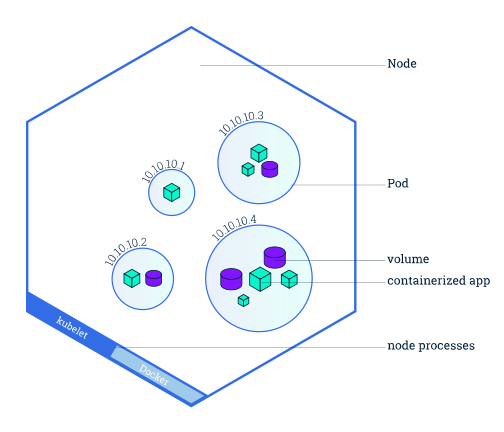
\includegraphics[width=0.7\linewidth]{Pics/nodes}
		\caption{\label{fig:nodes} Cấu tạo của Nodes.}
		\label{fig:nodes}
	\end{figure}
	
	\subsubsection{Quản lý}
	
	\hspace{1cm}{Có hai cách chính để thêm các Node vào máy chủ API:}
	
	\begin{enumerate}
		\item Kubelet trên một Node tự đăng ký vào control plane
		\item Thêm một đối tượng Node theo cách thủ công\\
	\end{enumerate}
	
	\hspace{0.3cm}{Sau khi bạn tạo một đối tượng Node hoặc kubelet trên Node tự đăng ký, control plane sẽ kiểm tra xem đối tượng Node mới có hợp lệ hay không. Ví dụ: nếu bạn cố gắng tạo một Node từ tệp kê khai JSON sau:\\}
	
	\begin{lstlisting}[language=Bash]
		{
			"kind": "Node",
			"apiVersion": "v1",
			"metadata": {
				"name": "10.240.79.157",
				"labels": {
					"name": "my-first-k8s-node"
				}
			}
		}
	\end{lstlisting}
	\smallskip
	
	\hspace{0.3cm}{Kubernetes tạo một đối tượng Node nội bộ. Kubernetes kiểm tra xem kubelet đã đăng ký với máy chủ API khớp với trường \texttt{metadata.name} của ứng dụng Node. Nếu Node hoạt động tốt (tức là tất cả các dịch vụ cần thiết đang chạy), thì Node đó đủ điều kiện để chạy Pod. Nếu không, Node đó sẽ bị bỏ qua đối với mọi hoạt động của cụm cho đến khi nó hoạt động bình thường.\\}
	
	\hspace{0.3cm}{Tên của một đối tượng Node phải là một tên miền phụ DNS hợp lệ.}
	
	\begin{itemize}
		\item \textbf{Tính duy nhất của tên Node}
		\smallskip
		\subitem Tên xác định một Node. Hai Node không thể có cùng tên cùng một lúc. Kubernetes cũng giả định rằng một tài nguyên có cùng tên là cùng một đối tượng. Trong trường hợp một Node, người ta mặc nhiên cho rằng một thể hiện sử dụng cùng tên sẽ có cùng trạng thái (ví dụ: cài đặt mạng, nội dung đĩa gốc) và các thuộc tính như nhãn Node. Điều này có thể dẫn đến sự không nhất quán nếu một phiên bản được sửa đổi mà không thay đổi tên của nó. Nếu Node cần được thay thế hoặc cập nhật đáng kể, đối tượng Node hiện có cần được xóa khỏi máy chủ API trước và thêm lại sau khi cập nhật.
		\smallskip
		\item \textbf{Tự đăng ký Node}
		\smallskip
		\subitem Khi cờ kubelet \texttt{--register-node} là \texttt{true} (mặc định), kubelet sẽ cố gắng tự đăng ký với máy chủ API. Đây là mẫu ưa thích, được sử dụng bởi hầu hết các bản phân phối.
		\smallskip
		\subitem Để tự đăng ký, kubelet được bắt đầu với các tùy chọn sau:
		
		\begin{itemize}
			\item \texttt{-kubeconfig} Đường dẫn đến thông tin đăng nhập để tự xác thực với máy chủ API.
			\item \texttt{-cloud-provider} Nói chuyện với một nhà cung cấp đám mây để đọc siêu dữ liệu về chính nó.
			\item \texttt{-register-node} Tự động đăng ký với máy chủ API.
			\item \texttt{-register-with-taints} Đăng ký Node với danh sách Taints đã cho (phân cách bằng dấu phẩy \texttt{<key>=<value>:<effect>}).
			
			No-op nếu \texttt{register-node} là sai.
			
			\item \texttt{-node-ip} Địa chỉ IP của Node.
			\item \texttt{-node-labels} - nhãn để thêm khi đăng ký Node trong cụm.
			\item \texttt{-node-status-update-frequency} Chỉ định tần suất kubelet đăng trạng thái Node của nó lên máy chủ API.
		\end{itemize}
		\smallskip
		\item \textbf{Quản lý Node thủ công}
		\smallskip
		\subitem Có thể tạo và sửa đổi các đối tượng Node bằng cách sử dụng kubectl.
		\smallskip
		\subitem Khi muốn tạo các đối tượng Node theo cách thủ công, hãy đặt cờ kubelet     \texttt{--register-node=false}.
		\smallskip
		\subitem Có thể sửa đổi các đối tượng Node bất kể cài đặt của \texttt{--register-node}. Ví dụ: bạn có thể đặt nhãn trên một Node hiện có hoặc đánh dấu Node đó là không thể lập lịch trình.
		\smallskip
		\subitem Có thể sử dụng nhãn trên Node kết hợp với bộ chọn Node trên Pod để kiểm soát việc lên lịch. Ví dụ: bạn có thể hạn chế một Pod chỉ đủ điều kiện chạy trên một tập hợp con các Nod có sẵn.
		\smallskip
		\subitem Việc đánh dấu một Node là không thể lập lịch trình sẽ ngăn bộ lập lịch đặt các Pod mới vào Node đó nhưng không ảnh hưởng đến các Pod hiện có trên Node. Điều này hữu ích như một bước chuẩn bị trước khi khởi động lại Node hoặc bảo trì khác.
		\subitem Để đánh dấu một Node không thể lên lịch, hãy chạy:\\
		\shellcmd{kubectl cordon \$NODENAME}
	\end{itemize}
	\subsubsection{Trạng thái Node}
	
	\hspace{1cm}{Trạng thái của Node chứa các thông tin sau:}
	\begin{enumerate}
		\item Địa chỉ
		\item Các điều kiện
		\item Năng lực và phân bổ
		\item Thông tin
	\end{enumerate}
	\smallskip
	\hspace{1cm}{Bạn có thể sử dụng \texttt{kubectl} để xem trạng thái của Node và các chi tiết khác.}
	
	\begin{itemize}
		\item \textbf{Địa chỉ}
		\smallskip
		\subitem Việc sử dụng các trường này khác nhau tùy thuộc vào nhà cung cấp dịch vụ đám mây hoặc cấu hình bare-metal.
		\begin{itemize}
			\item Tên máy chủ: Tên máy chủ được báo cáo bởi nhân của Node. Có thể được ghi đè thông qua tham số kubelet \texttt{-hostname-override}.
			\item IP bên ngoài: Điển hình là địa chỉ IP của Node có thể định tuyến bên ngoài (có sẵn từ bên ngoài cụm).
			\item InternalIP: Thông thường, địa chỉ IP của Node chỉ có thể định tuyến được trong cụm.
		\end{itemize}
		\smallskip
		\item \textbf{Các điều kiện}
		\smallskip
		\subitem Trường \texttt{conditions} mô tả trạng thái của tất cả các Node \texttt{Running}. Ví dụ về các điều kiện bao gồm:
		\begin{figure}
			\centering
			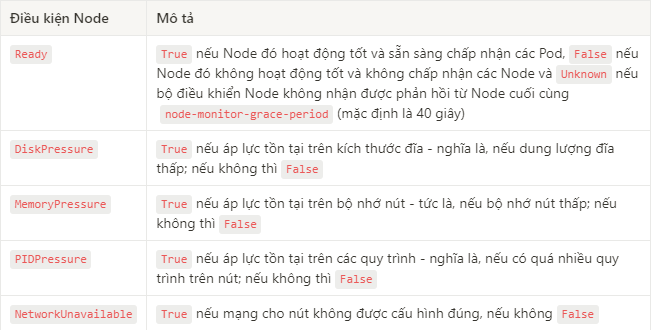
\includegraphics[width=1\linewidth]{Pics/conditions}
			\caption{\label{fig:conditions}Ví dụ về các điều kiện}
			\label{fig:conditions}
		\end{figure}
		\smallskip
		\subitem Trong API Kubernetes, điều kiện của Node được biểu diễn như một phần của \texttt{.status} của tài nguyên Node. Ví dụ: cấu trúc JSON sau đây mô tả một Node hoạt động tốt:
		\smallskip
		\begin{lstlisting}[language=Bash]
			"conditions": [
			{
				"type": "Ready",
				"status": "True",
				"reason": "KubeletReady",
				"message": "kubelet is posting ready status",
				"lastHeartbeatTime": "2019-06-05T18:38:35Z",
				"lastTransitionTime": "2019-06-05T11:41:27Z"
			}
			]
		\end{lstlisting}
		\smallskip
		\subitem Nếu \texttt{status} của Readly vẫn còn tình trạng \texttt{Unknown} hoặc \texttt{False} lâu hơn pod-eviction-timeout (một đối số được chuyển đến kube-controller-manager), thì bộ điều khiển Node sẽ kích hoạt quá trình do khởi tạo API trục xuất cho tất cả các Pod được gán cho Node đó. Thời gian chờ trục xuất mặc định là năm phút. Trong một số trường hợp khi không thể truy cập Node, máy chủ API không thể giao tiếp với kubelet trên Node. Quyết định xóa các Pod không thể được thông báo tới kubelet cho đến khi giao tiếp với máy chủ API được thiết lập lại. Trong thời gian chờ đợi, các Pod được lên lịch xóa có thể tiếp tục chạy trên Node được phân vùng.
		\smallskip
		\subitem Bộ điều khiển nút không buộc xóa các Pod cho đến khi được xác nhận rằng chúng đã ngừng chạy trong cụm. Có thể thấy các Nhóm có thể đang chạy trên một Node không thể truy cập được ở trạng thái \texttt{Terminating} hoặc \texttt{Unknown}. Trong trường hợp Kubernetes không thể suy luận từ cơ sở hạ tầng cơ bản nếu một Node đã rời khỏi cụm vĩnh viễn, quản trị viên cụm có thể cần phải xóa đối tượng Node bằng tay. Việc xóa đối tượng Node khỏi Kubernetes sẽ khiến tất cả các đối tượng Pod đang chạy trên Node bị xóa khỏi máy chủ API và giải phóng tên của chúng.
		\smallskip
		\subitem Khi xảy ra sự cố trên các Node, mặt phẳng điều khiển Kubernetes sẽ tự động tạo các dấu vết phù hợp với các điều kiện ảnh hưởng đến Node. Bộ lập lịch xem xét các yếu tố của Node khi gán một Pod cho một Node. Các Pod cũng có thể có dung sai cho phép chúng chạy trên một Node mặc dù nó có một taint cụ thể.
		\smallskip
		\item \textbf{Năng lực và phân bổ}
		\smallskip
		\subitem Mô tả các tài nguyên có sẵn trên Node: CPU, bộ nhớ và số lượng Pod tối đa có thể được lên lịch trên Node.
		\smallskip
		\subitem Các trường trong khối dung lượng cho biết tổng lượng tài nguyên mà một Node có. Khối có thể phân bổ cho biết lượng tài nguyên trên một Node có sẵn để các Pod thông thường sử dụng.
		\smallskip
		\item \textbf{Thông tin}
		\smallskip
		\subitem Mô tả thông tin chung về Node, chẳng hạn như phiên bản kernel, phiên bản Kubernetes (phiên bản kubelet và kube-proxy), chi tiết container runtime và hệ điều hành mà Node sử dụng. Kubelet thu thập thông tin này từ Node và xuất bản nó vào API Kubernetes.
	\end{itemize}
	
	\subsubsection{Heartbeats}
	
	\hspace{1cm}{Heartbeats, được gửi bởi các Node Kubernetes, giúp cụm xác định tính khả dụng của từng Node và thực hiện hành động khi phát hiện lỗi.\\}
	
	\hspace{0.3cm}{Đối với các Node có hai dạng Heartbeats:}
	\begin{itemize}
		\item cập nhật cho \texttt{.status} của một Node.
		\item Lease: Cho các đối tượng Node mượn trong không gian tên \texttt{kube-node-lease}. Mỗi Node có một đối tượng cho mượn được liên kết.
	\end{itemize}
	\hspace{0.3cm}{So với các bản cập nhật \texttt{.status} của Node, Lease là một tài nguyên nhẹ. Sử dụng Lease cho Heartbeats làm giảm tác động hiệu suất của các bản cập nhật này cho các cụm lớn.\\}
	
	\hspace{0.3cm}{Kubelet chịu trách nhiệm tạo và cập nhật các \texttt{.status} Node cũng như cập nhật các Lease liên quan của chúng.}
	
	\begin{itemize}
		\item Kubelet cập nhật \texttt{.status} của Node khi có thay đổi về trạng thái hoặc nếu không có bản cập nhật nào trong khoảng thời gian đã định cấu hình. Khoảng thời gian mặc định để cập nhật các Node là 5 phút, lâu hơn nhiều so với thời gian chờ mặc định 40 giây cho các Node không thể truy cập.
		\item Kubelet tạo và sau đó cập nhật đối tượng Lease của nó cứ sau 10 giây (khoảng thời gian cập nhật mặc định). Các bản cập nhật Lease xảy ra độc lập với các bản cập nhật cho \texttt{.status} của Node. Nếu cập nhật Lease không thành công, kubelet sẽ thử lại, sử dụng tính năng dự phòng theo cấp số nhân bắt đầu ở 200 mili giây và giới hạn ở 7 giây.
	\end{itemize}
	\subsubsection{Bộ điều khiển Node}
	
	\hspace{1cm}{Bộ điều khiển Node là một thành phần control plane Kubernetes quản lý các khía cạnh khác nhau của các Node.\\}
	
	\hspace{0.3cm}{Bộ điều khiển Node có nhiều vai trò trong vòng đời của Node. Đầu tiên là gán một khối CIDR cho Node khi nó được đăng ký (nếu chức năng gán CIDR được bật).\\}
	
	\hspace{0.3cm}{Thứ hai là giữ cho danh sách các Node nội bộ của bộ điều khiển Node được cập nhật với danh sách các máy có sẵn của nhà cung cấp đám mây. Khi chạy trong môi trường đám mây và bất cứ khi nào một Node không hoạt động tốt, bộ điều khiển Node sẽ hỏi nhà cung cấp đám mây xem VM cho Node đó có còn khả dụng hay không. Nếu không, bộ điều khiển Node sẽ xóa Node đó khỏi danh sách các Node của nó.\\}
	
	\hspace{0.3cm}{	Thứ ba là theo dõi tình trạng của các Node. Bộ điều khiển Node chịu trách nhiệm:}
	
	\begin{itemize}
		\item Trong trường hợp một Node không thể truy cập được, hãy cập nhật điều kiện trong trường \texttt{Ready} của \texttt{.status} Node. Trong trường hợp này, bộ điều khiển Node đặt điều kiện thành \texttt{Unknown}.
		\item Nếu một nút vẫn không thể truy cập: kích hoạt khởi tạo API trục xuất cho tất cả các Pod trên Node không thể truy cập. Theo mặc định, bộ điều khiển Node đợi 5 phút kể từ khi đánh dấu Node là \texttt{Unknown} và gửi yêu cầu trục xuất đầu tiên.
	\end{itemize}
	
	\hspace{0.3cm}{Theo mặc định, bộ điều khiển Node sẽ kiểm tra trạng thái của từng Node sau mỗi 5 giây. Khoảng thời gian này có thể được cấu hình bằng cách sử dụng cờ \texttt{--node-monitor-period} trên thành phần \texttt{kube-controller-manager}.}
	
	\subsection{Giao tiếp giữa các Node và Control Plane}
	
	\hspace{1cm}{Các giao tiếp bao gồm các đường dẫn giao tiếp giữa máy chủ API và cụm Kubernetes. Mục đích là cho phép người dùng tùy chỉnh cài đặt của họ để củng cố cấu hình mạng sao cho cụm có thể chạy trên mạng không đáng tin cậy (hoặc trên các IP công khai hoàn toàn trên nhà cung cấp dịch vụ đám mây).}
	
	\subsubsection{Node tới Control Plane}
	
	\hspace{1cm}{Kubernetes có mẫu API "hub-and-spoke". Tất cả việc sử dụng API từ các Node (hoặc Pod mà chúng chạy) sẽ chấm dứt tại máy chủ API. Không có thành phần Control plane nào khác được thiết kế để hiển thị các dịch vụ từ xa. Máy chủ API được định cấu hình để lắng nghe các kết nối từ xa trên cổng HTTPS an toàn (thường là 443) có bật một hoặc nhiều hình thức xác thực ứng dụng khách . Một hoặc nhiều hình thức ủy quyền phải được bật, đặc biệt nếu các yêu cầu ẩn danh hoặc mã thông báo tài khoản dịch vụ được cho phép.\\}
	
	\hspace{0.3cm}{Các Node phải được cung cấp chứng chỉ gốc công khai cho cụm sao cho chúng có thể kết nối an toàn với máy chủ API cùng với thông tin đăng nhập hợp lệ của ứng dụng khách. Một cách tiếp cận tốt là thông tin xác thực ứng dụng khách được cung cấp cho kubelet ở dạng chứng chỉ ứng dụng khách.\\}
	
	\hspace{0.3cm}{Các Pod muốn kết nối với máy chủ API có thể thực hiện việc này một cách an toàn bằng cách tận dụng tài khoản dịch vụ để Kubernetes sẽ tự động thêm chứng chỉ gốc công khai và mã thông báo hợp lệ vào nhóm khi nó được khởi tạo. Dịch vụ \texttt{kubernetes} (trong không gian tên \texttt{default}) được định cấu hình với một địa chỉ IP ảo được chuyển hướng (thông qua \texttt{kube-proxy}) đến điểm cuối HTTPS trên máy chủ API.\\}
	
	\hspace{0.3cm}{Các thành phần của control plane cũng giao tiếp với máy chủ API qua cổng an toàn.\\}
	
	\hspace{0.3cm}{Do đó, chế độ hoạt động mặc định cho các kết nối từ các Node và Pod chạy trên các Node đến Control plane được bảo mật theo mặc định và có thể chạy trên các mạng công cộng và/hoặc không đáng tin cậy.}
	
	\subsubsection{Control plane tới node}
	
	\hspace{1cm}{Có hai đường dẫn giao tiếp chính từ Control plane (máy chủ API) đến các Node. Đầu tiên là từ máy chủ API đến quy trình kubelet chạy trên mỗi Node trong cụm. Thứ hai là từ máy chủ API đến bất kỳ Node, Pod hoặc Service nào thông qua chức năng proxy của máy chủ API.}
	
	\begin{itemize}
		\item \textbf{API server đến kubelet}
		\smallskip
		\subitem Các kết nối từ máy chủ API đến kubelet được sử dụng cho:
		\begin{itemize}
			\item Tìm nạp nhật ký cho Pod.
			\item Đính kèm (thường thông qua \texttt{kubectl}) vào các Pod đang chạy.
			\item Cung cấp chức năng chuyển tiếp cổng của kubelet.
		\end{itemize}
		\subitem Các kết nối này kết thúc tại điểm cuối HTTPS của kubelet. Theo mặc định, máy chủ API không xác minh chứng chỉ phục vụ của kubelet, điều này làm cho kết nối phải chịu các cuộc tấn công trung gian và không an toàn khi chạy trên các mạng công cộng và/hoặc không đáng tin cậy.
		\smallskip
		\subitem Để xác minh kết nối này, hãy sử dụng cờ \texttt{--kubelet-certificate-authority} để cung cấp cho máy chủ API gói chứng chỉ gốc nhằm sử dụng để xác minh chứng chỉ cung cấp của kubelet.
		\smallskip
		\subitem Nếu không thể, hãy sử dụng đường hầm SSH giữa máy chủ API và kubelet nếu cần để tránh kết nối qua mạng công cộng hoặc không đáng tin cậy.
		\smallskip
		\subitem Cuối cùng, xác thực và/hoặc ủy quyền Kubelet phải được bật để bảo mật API kubelet.
		
		\item \textbf{API server đến các Node, Pod hoặc Service}
		\smallskip
		\subitem Các kết nối từ máy chủ API đến một Node, Pod hoặc Service mặc định là kết nối HTTP đơn giản và do đó không được xác thực cũng như không được mã hóa. Chúng có thể được chạy qua kết nối HTTPS an toàn bằng cách thêm tiền tố \texttt{https:} vào tên Node, Pod hoặc Service trong URL API, nhưng chúng sẽ không xác thực chứng chỉ do điểm cuối HTTPS cung cấp cũng như không cung cấp thông tin đăng nhập của khách hàng. Vì vậy, mặc dù kết nối sẽ được mã hóa nhưng nó sẽ không cung cấp bất kỳ đảm bảo nào về tính toàn vẹn. Các kết nối này hiện không an toàn để chạy qua các mạng công cộng hoặc không đáng tin cậy.
		
		\item \textbf{SSH tunnels}
		\smallskip
		\subitem Kubernetes hỗ trợ các SSH tunnel để bảo vệ các đường dẫn giao tiếp của control plane đến Node. Trong cấu hình này, máy chủ API khởi tạo một SSH tunnel tới từng Node trong cụm (kết nối với máy chủ SSH đang nghe trên cổng 22) và chuyển tất cả lưu lượng dành cho kubelet, Node, Pod hoặc Service qua tunnel. Tunnel này đảm bảo rằng lưu lượng không bị lộ ra bên ngoài mạng mà các Node đang chạy.
		\smallskip
		\subitem \textbf{Lưu ý}: SSH tunnel hiện không được dùng nữa, vì vậy không nên chọn sử dụng chúng trừ khi biết bản thân đang sử dụng với mục đích gì. Dịch vụ Konnectivity là sự thay thế cho kênh liên lạc này.
		
		\item \textbf{Dịch vụ Konnectivity}
		\smallskip
		\subitem Để thay thế cho các SSH tunnel, dịch vụ Konnectivity cung cấp proxy cấp TCP cho mặt phẳng điều khiển để liên lạc theo cụm. Dịch vụ Konnectivity bao gồm hai phần: máy chủ Konnectivity trong mạng control plane và tác nhân Konnectivity trong mạng Node. Tác nhân Konnectivity khởi tạo kết nối đến máy chủ Konnectivity và duy trì kết nối mạng. Sau khi kích hoạt dịch vụ Konnectivity, tất cả lưu lượng truy cập từ control plane đến các Node đều đi qua các kết nối này.
	\end{itemize}

	\subsection{Controllers}
	
	\hspace{1cm}{Trong chế tạo rô-bốt và tự động hóa, vòng lặp điều khiển là một vòng lặp không kết thúc điều chỉnh trạng thái của hệ thống.\\}
	
	\hspace{0.3cm}{\textbf{Ví dụ}: bộ điều chỉnh nhiệt trong phòng: Khi bạn đặt nhiệt độ, điều đó báo cho bộ điều chỉnh nhiệt về trạng thái mong muốn của bạn. Nhiệt độ phòng thực tế là trạng thái hiện tại. Bộ điều chỉnh nhiệt hoạt động để đưa trạng thái hiện tại đến gần trạng thái mong muốn hơn bằng cách bật hoặc tắt thiết bị.\\}
	
	\hspace{0.3cm}{Trong Kubernetes, bộ điều khiển là các vòng điều khiển theo dõi trạng thái trong cụm, sau đó thực hiện hoặc yêu cầu thay đổi nếu cần. Mỗi bộ điều khiển cố gắng di chuyển trạng thái cụm hiện tại đến gần trạng thái mong muốn hơn.}
	
	\subsubsection{Kiểu điều khiển}
	
	\hspace{1cm}{Bộ điều khiển theo dõi ít nhất một loại tài nguyên Kubernetes. Các đối tượng này có một trường thông số đại diện cho trạng thái mong muốn. (Các) bộ điều khiển cho tài nguyên đó chịu trách nhiệm làm cho trạng thái hiện tại tiến gần hơn đến trạng thái mong muốn đó.\\}
	
	\hspace{0.3cm}{Bộ điều khiển có thể tự thực hiện hành động; thông thường hơn, trong Kubernetes, bộ điều khiển sẽ gửi tin nhắn đến máy chủ API có tác dụng phụ hữu ích.}
	
	\begin{itemize}
		\item \textbf{Điều khiển thông qua máy chủ API}
		\smallskip
		\subitem Công việc của bộ điều khiển là một ví dụ về bộ điều khiển tích hợp Kubernetes. Bộ điều khiển tích hợp quản lý trạng thái bằng cách tương tác với máy chủ API cụm.
		\smallskip
		\subitem Công việc là một tài nguyên Kubernetes chạy một Pod, hoặc có thể là một số Pod, để thực hiện một tác vụ rồi dừng lại.
		\smallskip
		\subitem (Sau khi được lên lịch , các đối tượng Pod trở thành một phần của trạng thái mong muốn cho một kubelet).
		\smallskip
		\subitem Khi bộ điều khiển Công việc nhìn thấy một tác vụ mới, nó đảm bảo rằng, ở đâu đó trong cụm của bạn, các kubelet trên một nhóm các Node đang chạy đúng số lượng Pod để hoàn thành công việc. Bộ điều khiển công việc không tự chạy bất kỳ các Pod hoặc Container nào. Thay vào đó, bộ điều khiển Công việc yêu cầu máy chủ API tạo hoặc xóa Pod. Các thành phần khác trong control plane hành động dựa trên thông tin mới (có các Pod mới để lên lịch và chạy), và cuối cùng công việc đã hoàn thành.
		\smallskip
		\subitem Sau khi bạn tạo một Công việc mới, trạng thái mong muốn là Công việc đó đã được hoàn thành. Bộ điều khiển Công việc làm cho trạng thái hiện tại của Công việc đó gần với trạng thái mong muốn hơn: tạo các Pod thực hiện làm việc cho Công việc đó, để Công việc gần hoàn thành hơn.
		\smallskip
		\subitem Bộ điều khiển cũng cập nhật các đối tượng cấu hình chúng. Ví dụ: sau khi hoàn thành việc làm cho một Công việc, bộ điều khiển Công việc sẽ cập nhật đối tượng Công việc đó để đánh dấu nó \texttt{Finished}.
		
		\item \textbf{Điều khiển trực tiếp}
		\smallskip
		\subitem Ngược lại với Công việc, một số bộ điều khiển cần thực hiện thay đổi đối với những thứ bên ngoài cụm.
		\smallskip
		\subitem \textbf{Ví dụ}: nếu bạn sử dụng vòng lặp điều khiển để đảm bảo có đủ các Node trong cụm của bạn, thì bộ điều khiển đó cần thứ gì đó bên ngoài cụm hiện tại để thiết lập các Node mới khi cần.
		\smallskip
		\subitem Các bộ điều khiển tương tác với trạng thái bên ngoài sẽ tìm thấy trạng thái mong muốn của chúng từ máy chủ API, sau đó giao tiếp trực tiếp với hệ thống bên ngoài để đưa trạng thái hiện tại đến gần trạng thái mong muốn hơn.
		\smallskip
		\subitem (Thực sự có một bộ điều khiển chia tỷ lệ các nút trong cụm của bạn theo chiều ngang.)
		\smallskip
		\subitem Điểm quan trọng ở đây là bộ điều khiển thực hiện một số thay đổi để mang lại trạng thái mong muốn, sau đó báo cáo trạng thái hiện tại trở lại máy chủ API của cụm. Các vòng điều khiển khác có thể quan sát dữ liệu được báo cáo đó và thực hiện các hành động của riêng chúng.
		\smallskip
		\subitem Với các cụm Kubernetes, control plane hoạt động gián tiếp với các công cụ quản lý địa chỉ IP, dịch vụ lưu trữ, API của nhà cung cấp đám mây và các dịch vụ khác bằng cách mở rộng Kubernetes để triển khai điều đó.
	\end{itemize}
	\subsubsection{Mong muốn so với trạng thái hiện tại}
	
	\hspace{1cm}{Kubernetes có chế độ xem hệ thống dựa trên đám mây và có thể xử lý thay đổi liên tục.\\}
	
	\hspace{0.3cm}{Cụm của bạn có thể thay đổi bất kỳ lúc nào khi công việc diễn ra và các vòng lặp điều khiển sẽ tự động khắc phục lỗi. Điều này có nghĩa là, có khả năng, cụm của bạn không bao giờ đạt đến trạng thái ổn định.\\}
	
	\hspace{0.3cm}{Miễn là các bộ điều khiển cho cụm đang chạy và có thể thực hiện các thay đổi hữu ích, nó không quan trọng nếu trạng thái tổng thể là ổn định hay không.}
	
	\subsubsection{Thiết kế}
	
	\hspace{1cm}{Như một nguyên lý trong thiết kế của nó, Kubernetes sử dụng rất nhiều bộ điều khiển mà mỗi bộ điều khiển quản lý một khía cạnh cụ thể của trạng thái cụm. Thông thường nhất, một vòng lặp điều khiển cụ thể (bộ điều khiển) sử dụng một loại tài nguyên làm trạng thái mong muốn của nó và có một loại tài nguyên khác mà nó quản lý để thực hiện trạng thái mong muốn đó. Ví dụ: bộ điều khiển cho Công việc theo dõi các đối tượng Công việc (để khám phá công việc mới) và các đối tượng Pod (để chạy Công việc, sau đó để xem khi nào công việc kết thúc). Trong trường hợp này, một cái gì đó khác tạo ra Công việc, trong khi bộ điều khiển Công việc tạo ra các Pod.\\}
	
	\hspace{0.3cm}{Thật hữu ích khi có các bộ điều khiển đơn giản thay vì một bộ vòng điều khiển nguyên khối được liên kết với nhau. Bộ điều khiển có thể bị lỗi, vì vậy Kubernetes được thiết kế để cho phép điều đó xảy ra.\\}
	
	\hspace{0.3cm}{\textbf{Ghi chú}: Có thể có một số bộ điều khiển tạo hoặc cập nhật cùng một loại đối tượng. Đằng sau hậu trường, bộ điều khiển Kubernetes đảm bảo rằng họ chỉ chú ý đến các tài nguyên được liên kết với tài nguyên kiểm soát của họ.\\}
	
	\hspace{0.3cm}{\textbf{Ví dụ}: bạn có thể có các Deployment và Công việc; cả hai đều tạo ra các Pod. Bộ điều khiển công việc không xóa các Pod mà Deployment của bạn đã tạo, vì có thông tin (nhãn) bộ điều khiển có thể sử dụng để phân biệt các Pod đó.}
	
	\subsubsection{Các cách chạy bộ điều khiển}
	
	\hspace{1cm}{Kubernetes đi kèm với một bộ điều khiển tích hợp chạy bên trong kube-controller-manager. Các bộ điều khiển tích hợp này cung cấp các hành vi cốt lõi quan trọng.\\}
	
	\hspace{0.3cm}{Bộ điều khiển Deployment và Bộ điều khiển công việc là những ví dụ về bộ điều khiển là một phần của chính Kubernetes (bộ điều khiển "tích hợp"). Kubernetes cho phép bạn chạy một control plane có khả năng đối phó để nếu bất kỳ bộ điều khiển tích hợp nào bị lỗi, một phần khác của control plane sẽ đảm nhận công việc.\\}
	
	\hspace{0.3cm}{Bạn có thể tìm các bộ điều khiển chạy bên ngoài control plane để mở rộng Kubernetes. Hoặc, nếu muốn, bạn có thể tự viết một bộ điều khiển mới. Bạn có thể chạy bộ điều khiển của riêng mình dưới dạng một bộ Pod hoặc bên ngoài Kubernetes. Những gì phù hợp nhất sẽ phụ thuộc vào chức năng của bộ điều khiển cụ thể đó.}
	
	\subsection{Quản lý controller cloud}
	
	\hspace{1cm}{Các công nghệ cơ sở hạ tầng đám mây cho phép bạn chạy Kubernetes trên các đám mây công cộng, riêng tư và lai. Kubernetes tin tưởng vào tự động hóa, dựa trên cơ sở hạ tầng API mà không cần sự liên kết chặt chẽ giữa các thành phần.\\}
	
	\hspace{0.3cm}{Trình quản lý bộ điều khiển đám mây là một thành phần control plane Kubernetes nhúng logic điều khiển dành riêng cho đám mây. Trình quản lý bộ điều khiển đám mây cho phép bạn liên kết cụm của mình với API của nhà cung cấp đám mây và tách các thành phần tương tác với nền tảng đám mây đó khỏi các thành phần chỉ tương tác với cụm của bản thân.\\}
	
	\hspace{0.3cm}{Bằng cách tách logic khả năng tương tác giữa Kubernetes và cơ sở hạ tầng đám mây cơ bản, thành phần trình quản lý điều khiển đám mây cho phép các nhà cung cấp đám mây phát hành các tính năng ở một tốc độ khác so với dự án Kubernetes chính.\\}
	
	\hspace{0.3cm}{Cloud-controller-manager được cấu trúc bằng cơ chế plugin cho phép các nhà cung cấp đám mây khác nhau tích hợp nền tảng của họ với Kubernetes.}
	
	\subsubsection{Thiết kế}
	
	\hspace{1cm}{Trình quản lý bộ điều khiển đám mây chạy trong control plane dưới dạng một tập hợp các quy trình được sao chép (thông thường, đây là các bộ chứa trong Pod). Mỗi cloud-controller-manager thực hiện nhiều bộ điều khiển trong một quy trình duy nhất.\\}
	
	\hspace{0.3cm}{\textbf{Lưu ý}: Bạn cũng có thể chạy trình quản lý bộ điều khiển đám mây dưới dạng Kubernetes thêm vào chứ không phải là một phần của contol plane.}
	
	\subsubsection{Chức năng quản lý bộ điều khiển đám mây}
	
	\hspace{1cm}{Các bộ điều khiển bên trong trình quản lý bộ điều khiển đám mây bao gồm:}
	
	\begin{itemize}
		\item \textbf{Bộ điều khiển Node}
		\smallskip
		\subitem Bộ điều khiển nút chịu trách nhiệm cập nhật các đối tượng Node khi máy chủ mới được tạo trong cơ sở hạ tầng đám mây của bạn. Bộ điều khiển Node lấy thông tin về các máy chủ đang chạy bên trong nơi bạn thuê với nhà cung cấp đám mây. Bộ điều khiển nút thực hiện các chức năng sau:
		\begin{enumerate}
			\item Cập nhật một đối tượng Node với mã định danh duy nhất của máy chủ tương ứng thu được từ API của nhà cung cấp đám mây.
			\item Chú thích và gắn nhãn cho đối tượng Nút bằng thông tin dành riêng cho đám mây, chẳng hạn như khu vực mà nút được triển khai và các tài nguyên (CPU, bộ nhớ, v.v.) mà nút có sẵn.
			\item Lấy tên máy chủ và địa chỉ mạng của Node.
			\item Xác minh tình trạng của Node. Trong trường hợp một Node không phản hồi, bộ điều khiển này sẽ kiểm tra với API của nhà cung cấp dịch vụ đám mây của bạn để xem máy chủ đã bị hủy kích hoạt/xóa/chấm dứt chưa. Nếu Node đã bị xóa khỏi đám mây, bộ điều khiển sẽ xóa đối tượng Node khỏi cụm Kubernetes.
		\end{enumerate}
		\smallskip
		\subitem Một số triển khai của nhà cung cấp đám mây chia phần này thành bộ điều khiển Node và bộ điều khiển vòng đời Node riêng biệt.
		\smallskip
		\item \textbf{Bộ điều khiển định tuyến}
		\smallskip
		\subitem Bộ điều khiển định tuyến chịu trách nhiệm định cấu hình các tuyến đường trong đám mây một cách thích hợp để các vùng chứa trên các Node khác nhau trong cụm Kubernetes có thể giao tiếp với nhau.
		\smallskip
		\subitem Tùy thuộc vào nhà cung cấp đám mây, bộ điều khiển định tuyến cũng có thể phân bổ các khối địa chỉ IP cho mạng Pod.
		\smallskip
		\item \textbf{Bộ điều khiển dịch vụ}
		\smallskip
		\subitem Dịch vụ tích hợp với các thành phần cơ sở hạ tầng đám mây như bộ cân bằng tải được quản lý, địa chỉ IP, lọc gói mạng và kiểm tra tình trạng mục tiêu. Bộ điều khiển dịch vụ tương tác với API của nhà cung cấp dịch vụ đám mây để thiết lập bộ cân bằng tải và các thành phần cơ sở hạ tầng khác khi bản thân khai báo yêu cầu tài nguyên dịch vụ.
	\end{itemize}
	
	\subsubsection{Ủy quyền}
	
	\hspace{1cm}{Phần này chia nhỏ quyền truy cập mà trình quản lý bộ điều khiển đám mây yêu cầu trên các đối tượng API khác nhau để thực hiện các hoạt động của nó.}
	\begin{itemize}
		\item \textbf{Bộ điều khiển nút}
		\smallskip
		\subitem Bộ điều khiển Node chỉ hoạt động với các đối tượng Node. Nó yêu cầu toàn quyền truy cập để đọc và sửa đổi các đối tượng Node.
		\subitem \texttt{v1/Node}:
		\begin{itemize}
			\item Get
			\item List
			\item Create
			\item Update
			\item Patch
			\item Watch
			\item Delete
		\end{itemize}
		\item \textbf{Bộ điều khiển định tuyến}
		\smallskip
		\subitem Bộ điều khiển tuyến đường lắng nghe việc tạo đối tượng Node và định cấu hình các tuyến đường một cách thích hợp. Nó yêu cầu Nhận quyền truy cập vào các đối tượng Nút.
		\subitem \texttt{v1/Node}:
		\begin{itemize}
			\item Get
		\end{itemize}
		\item \textbf{Bộ điều khiển dịch vụ}
		\smallskip
		\subitem Bộ điều khiển dịch vụ lắng nghe các sự kiện Tạo, Cập nhật và Xóa đối tượng Dịch vụ, sau đó định cấu hình Điểm cuối cho các Dịch vụ đó một cách thích hợp (đối với EndpointSlices, trình quản lý bộ điều khiển kube quản lý các điểm cuối này theo yêu cầu).
		\smallskip
		\subitem Để truy cập Dịch vụ, nó yêu cầu quyền truy cập Danh sách và Xem. Để cập nhật Dịch vụ, nó yêu cầu quyền truy cập Bản vá và Cập nhật.
		\smallskip
		\subitem Để thiết lập tài nguyên Điểm cuối cho Dịch vụ, nó yêu cầu quyền truy cập vào Tạo, Liệt kê, Nhận, Xem và Cập nhật.
		\subitem \texttt{v1/Service}:
		\begin{itemize}
			\item List
			\item Get
			\item Watch
			\item Patch
			\item Update
		\end{itemize}
		\item \textbf{Khác}
		\smallskip
		\subitem Việc triển khai lõi của trình quản lý bộ điều khiển đám mây yêu cầu quyền truy cập để tạo đối tượng Sự kiện và để đảm bảo hoạt động an toàn, nó yêu cầu quyền truy cập để tạo Tài khoản dịch vụ.
		\subitem \texttt{v1/Event}:
		\begin{itemize}
			\item Create
			\item Patch
			\item Update
		\end{itemize}
		\subitem \texttt{v1/ServiceAccount}:
		\begin{itemize}
			\item Create
		\end{itemize}
	\end{itemize}
	\hspace{0.3cm}{Các RBAC(Kiểm soát truy cập dựa trên vai trò: là phương pháp điều chỉnh quyền truy cập vào máy tính hoặc tài nguyên mạng dựa trên vai trò của từng người dùng trong tổ chức) ClusterRole cho trình quản lý bộ điều khiển đám mây trông giống như:}
\begin{lstlisting}[language=Bash]
apiVersion: rbac.authorization.k8s.io/v1
kind: ClusterRole
metadata:
	name: cloud-controller-manager
rules:
	- apiGroups:
		- ""
		resources:
		- events
		verbs:
		- create
		- patch
		- update
	- apiGroups:
		- ""
		resources:
		- nodes
		verbs:
		- '*'
	- apiGroups:
		- ""
		resources:
		- nodes/status
		verbs:
		- patch
	- apiGroups:
		- ""
		resources:
		- services
		verbs:
		- list
		- patch
		- update
		- watch
	- apiGroups:
		- ""
		resources:
		- serviceaccounts
		verbs:
		- create
	- apiGroups:
		- ""
		resources:
		- persistentvolumes
		verbs:
		- get
		- list
		- update
		- watch
	- apiGroups:
		- ""
		resources:
		- endpoints
		verbs:
		- create
		- get
		- list
		- watch
		- update
\end{lstlisting}
	\section{Điểm mạnh của Kubenertes}
	\subsection{Điểm mạnh}
	
	\hspace{1cm}{Kubernetes là một nền tảng mã nguồn mở, di động, có thể mở rộng để quản lý khối lượng công việc và dịch vụ được container hóa, hỗ trợ cả cấu hình khai báo và tự động hóa. Nó có một hệ sinh thái lớn, phát triển nhanh chóng. Các dịch vụ, hỗ trợ và công cụ Kubernetes được phổ biến rộng rãi.\\}
	
	\hspace{0.3cm}{Container là một cách hay để đóng gói và chạy các ứng dụng của bạn. Trong môi trường sản xuất, bạn cần quản lý các Container chạy ứng dụng và đảm bảo rằng không có thời gian chết. Ví dụ: nếu một Container gặp sự cố, thì một Container khác cần phải khởi động. Sẽ không dễ dàng hơn nếu hành vi này được xử lý bởi một hệ thống?\\}
	
	\hspace{0.3cm}{Đó là cách Kubernetes hoạt động! Kubernetes cung cấp cho bạn một khung để chạy các hệ thống phân tán một cách linh hoạt. Nó đảm nhiệm việc mở rộng quy mô và chuyển đổi dự phòng cho ứng dụng của bạn, cung cấp các mẫu triển khai, v.v. Ví dụ: Kubernetes có thể dễ dàng quản lý triển khai canary cho hệ thống của bạn.\\}
	
	\hspace{0.3cm}{Kubenertes cung cấp cho bạn:}
	\begin{itemize}
		\item Phát hiện dịch vụ và cân bằng tải Kubernetes có thể hiển thị Container bằng cách sử dụng tên DNS hoặc sử dụng địa chỉ IP của chính chúng. Nếu lưu lượng truy cập vào Container cao, Kubernetes có thể cân bằng tải và phân phối lưu lượng mạng để quá trình triển khai ổn định.
		\item Điều phối lưu trữ Kubernetes cho phép bạn tự động gắn hệ thống lưu trữ mà bạn chọn, chẳng hạn như kho lưu trữ cục bộ, nhà cung cấp đám mây công cộng, v.v.
		\item Triển khai và khôi phục tự động bạn có thể mô tả trạng thái mong muốn cho các Container đã triển khai của mình bằng Kubernetes và nó có thể thay đổi trạng thái thực tế thành trạng thái mong muốn với tốc độ được kiểm soát. Ví dụ: bạn có thể tự động hóa Kubernetes để tạo Container mới cho quá trình triển khai của mình, xóa Container hiện có và áp dụng tất cả tài nguyên của chúng vào Container mới.
		\item Đóng gói thùng tự động Bạn cung cấp cho Kubernetes một cụm các nút mà nó có thể sử dụng để chạy các tác vụ Container. Bạn cho Kubernetes biết lượng CPU và bộ nhớ (RAM) mà mỗi Container cần. Kubernetes có thể lắp các Container vào các nút của bạn để tận dụng tốt nhất các tài nguyên của bạn.
		\item Kubernetes tự phục hồi khởi động lại các Container bị lỗi, thay thế các Container, hủy các Container không phản hồi kiểm tra tình trạng do người dùng xác định của bạn và không quảng cáo chúng cho khách hàng cho đến khi chúng sẵn sàng phân phối.
		\item Quản lý cấu hình và bí mật Kubernetes cho phép bạn lưu trữ và quản lý thông tin nhạy cảm, chẳng hạn như mật khẩu, mã thông báo OAuth và khóa SSH. Bạn có thể triển khai và cập nhật các bí mật cũng như cấu hình ứng dụng mà không cần xây dựng lại hình ảnh Container cũng như không để lộ bí mật trong cấu hình ngăn xếp của mình.
	\end{itemize}
	\subsection{Làm rõ tác dụng của Kubenertes}
	
	\hspace{1cm}{Kubernetes không phải là một hệ thống PaaS (Nền tảng dưới dạng dịch vụ) truyền thống, bao gồm tất cả. Vì Kubernetes hoạt động ở cấp vùng chứa thay vì ở cấp phần cứng, nên nó cung cấp một số tính năng có thể áp dụng chung cho các dịch vụ PaaS, chẳng hạn như triển khai, mở rộng quy mô, cân bằng tải và cho phép người dùng tích hợp các giải pháp ghi nhật ký, giám sát và cảnh báo của họ. Tuy nhiên, Kubernetes không phải là nguyên khối và các giải pháp mặc định này là tùy chọn và có thể cắm được. Kubernetes cung cấp các khối xây dựng để xây dựng nền tảng dành cho nhà phát triển, nhưng vẫn duy trì sự lựa chọn và tính linh hoạt của người dùng ở những nơi quan trọng.}
	\begin{itemize}
		\item Không giới hạn các loại ứng dụng được hỗ trợ. Kubernetes nhằm mục đích hỗ trợ khối lượng công việc cực kỳ đa dạng, bao gồm khối lượng công việc không trạng thái, trạng thái và xử lý dữ liệu. Nếu một ứng dụng có thể chạy trong Container, thì ứng dụng đó sẽ chạy tốt trên Kubernetes.
		\item Không triển khai mã nguồn và không xây dựng ứng dụng của bạn. Dòng công việc Tích hợp, Phân phối và Triển khai Liên tục (CI/CD) được xác định bởi văn hóa và sở thích của tổ chức cũng như các yêu cầu kỹ thuật.
		\item Không cung cấp dịch vụ cấp ứng dụng, chẳng hạn như phần mềm trung gian (ví dụ: bus thông báo), khung xử lý dữ liệu (ví dụ: Spark), cơ sở dữ liệu (ví dụ: MySQL), bộ đệm cũng như hệ thống lưu trữ cụm (ví dụ: Ceph) như các dịch vụ tích hợp. Các thành phần như vậy có thể chạy trên Kubernetes và/hoặc có thể được truy cập bởi các ứng dụng chạy trên Kubernetes thông qua các cơ chế di động, chẳng hạn như Open Service Broker.
		\item Không ra lệnh cho các giải pháp ghi nhật ký, giám sát hoặc cảnh báo. Nó cung cấp một số tích hợp làm bằng chứng về khái niệm và cơ chế để thu thập và xuất các số liệu.
		\item Không cung cấp cũng như không bắt buộc ngôn ngữ/hệ thống cấu hình (ví dụ: Jsonnet). Nó cung cấp một API khai báo có thể được nhắm mục tiêu bởi các dạng thông số kỹ thuật khai báo tùy ý.
		\item Không cung cấp cũng như áp dụng bất kỳ hệ thống cấu hình, bảo trì, quản lý hoặc tự phục hồi toàn diện nào của máy.
		\item Ngoài ra, Kubernetes không phải là một hệ thống điều phối đơn thuần. Trên thực tế, nó loại bỏ nhu cầu phối hợp. Định nghĩa kỹ thuật của điều phối là thực thi một quy trình công việc đã xác định: đầu tiên thực hiện A, sau đó là B, sau đó là C. Ngược lại, Kubernetes bao gồm một tập hợp các quy trình kiểm soát độc lập, có thể kết hợp, liên tục thúc đẩy trạng thái hiện tại hướng tới trạng thái mong muốn được cung cấp. Việc bạn đi từ A đến C bằng cách nào không quan trọng. Kiểm soát tập trung cũng không bắt buộc. Điều này dẫn đến một hệ thống dễ sử dụng hơn và mạnh mẽ hơn, mạnh mẽ hơn, linh hoạt hơn và có thể mở rộng.
	\end{itemize}


	\chapter{Giới thiệu về HashiCorp Vault}
	
	\section{Tổng quát về Vault}
	\hspace{1.0cm} {Hãy tưởng tượng rằng ai đó đang đi nghỉ ở một địa điểm đẹp và kỳ lạ. Chuyến đi của họ sẽ bắt đầu bằng việc họ đến khách sạn để nhận phòng. Tại quầy lễ tân, nhân viên tiếp tân yêu cầu người đó chứng minh danh tính của họ bằng cách cung cấp thông tin đăng nhập. Sau đó, nhân viên lễ tân sẽ kiểm tra thông tin đăng nhập của họ đối với hồ sơ khách sạn trong hồ sơ và xác định rằng họ chính là người mà họ nói. Sau khi xác minh danh tính của khách, lễ tân sẽ cấp cho khách chìa khóa phòng. Mức độ truy cập cụ thể được cấp cho khách sẽ phụ thuộc vào mối quan hệ của khách với khách sạn. Trong trường hợp khách đến lần đầu chỉ có thể được sử dụng phòng của họ và phòng tập thể dục của khách sạn, thì khách quay lại cũng có thể được sử dụng phòng chờ dành cho khách vì sự tin tưởng của họ.\\}
	
	\hspace{0.3cm}{Quy trình làm việc cho ứng dụng khách Vault giao tiếp với HashiCorp Vault tương tự như quy trình nhận phòng tại khách sạn. Giống như Vault, một khách sạn có nhiều lối vào để khách có thể vào sảnh đợi và phòng dành cho khách. Khi ứng dụng khách Vault cần quyền truy cập vào Vault, nó sẽ thực hiện điều đó thông qua nhiều giao diện khác nhau, bao gồm API mạnh mẽ, CLI và giao diện người dùng. Việc bảo vệ Vault được thực hiện thông qua hàng rào mật mã, tương tự như cách một khách sạn xây tường và cửa để bảo vệ các phòng và tiện nghi của khách. Hàng rào mật mã này chịu trách nhiệm mã hóa tất cả thông tin được lưu trữ bởi Vault.\\}
	
	\hspace{0.3cm}{Mục tiêu của khách hàng Vault là truy cập dữ liệu từ một công cụ bảo mật giống như cách khách hàng của chúng tôi truy cập vào phòng của họ. Tuy nhiên, trước khi ứng dụng khách Vault được phép truy cập vào một bí mật, ứng dụng đó phải xác thực với Vault để chứng minh danh tính của mình, giống như khách của chúng tôi phải đăng ký trước khi vào phòng của họ. Giống như bộ phận lễ tân kiểm tra ID của khách hàng, Vault xác thực thông tin đăng nhập của người dùng thông qua phương thức xác thực được định cấu hình để đảm bảo những thông tin đăng nhập đó hợp lệ. Sau khi xác thực thành công, Vault cấp mã thông báo cho khách hàng dựa trên chính sách đã xác định cho người dùng đó. Tương tự như chìa khóa phòng của khách cho phép họ truy cập vào các địa điểm khác nhau trong khách sạn, mã thông báo này (dựa trên chính sách đã xác định) cho phép ứng dụng khách Vault truy cập các điểm cuối khác nhau trong Vault, được gọi là đường dẫn. Mã thông báo có giá trị trong một khoảng thời gian đã đặt bằng cách sử dụng thời gian tồn tại (TTL) và không còn giá trị sau khi hết hạn, giống như khóa của khách sẽ không còn hoạt động khi thời gian lưu trú của họ kết thúc.\\ }
	
	\hspace{0.3cm}{Mặc dù các dịch vụ được phép này có thể không phải là phòng tập thể dục sang trọng hay phòng khách sang trọng, nhưng chúng có thể bao gồm truy xuất bí mật tĩnh, tạo thông tin xác thực mới hoặc mã hóa dữ liệu.}
	
	
<<<<<<< Updated upstream
	\subsection{Khái niệm về Vault}
=======
	\begin{figure}[h]
		\centering
		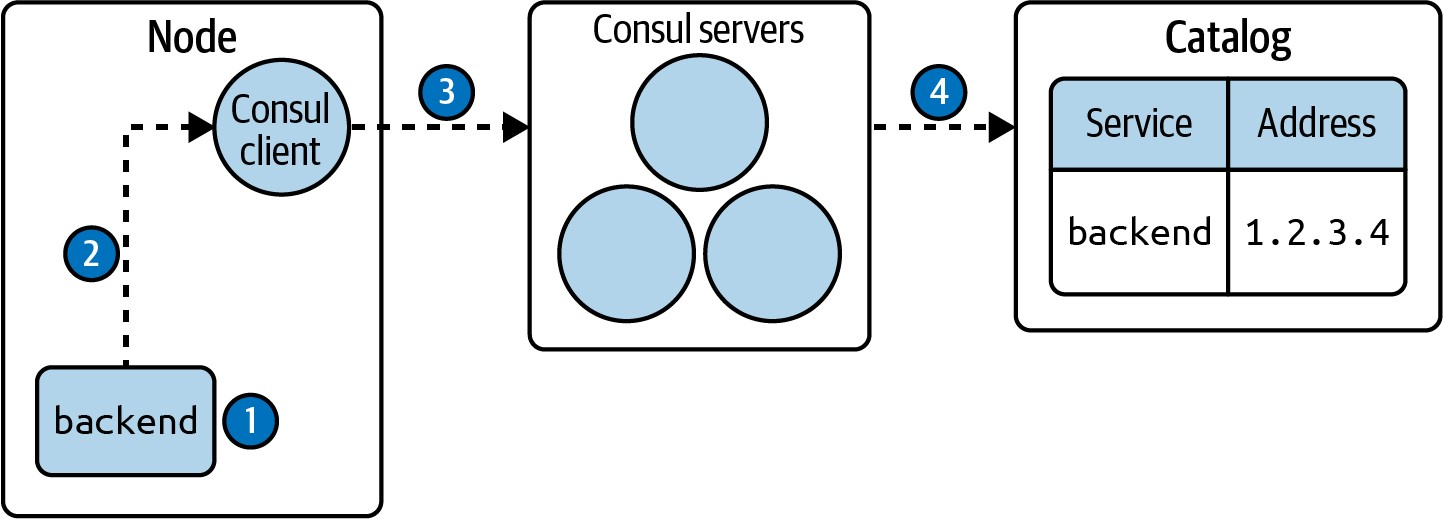
\includegraphics[width=0.7\linewidth]{Pics/example}
		\caption{\label{fig:example} Một dịch vụ mới đang được bắt đầu trên một Node.}
		\label{fig:example}
	\end{figure}
>>>>>>> Stashed changes
	
	\hspace{1.0cm}{HashiCorp Vault là một hệ thống các thông tin mã hoá và bí mật dựa trên danh tính. Một bí mật là thứ mà bạn muốn siết chặt quyền truy cập, như là khoá mã hoá API, mật khẩu và chứng chỉ. Vault cung cấp dịch vụ mã hoá mà kiểm soát bởi phương thức xác thực và xác minh. Sử dụng giao diện của Vault, câu lệnh hay là API, quyền truy cập vào các bí mật hay dữ liệu nhạy cảm khác được lưu trữ và quản lý an toàn, được kiểm soát chặt chẽ và có thể kiểm tra được.\\}
	
<<<<<<< Updated upstream
	\hspace{1.0cm}{Một hệ thống hiện đại yêu cầu quyền truy cập vào vô số bí mật, bao gồm thông tin đăng nhập cơ sở dữ liệu, khoá API cho các dịch vụ bên ngoài, etc... Có thể khó hiểu ai đang truy cập bí mật nào, đặc biệt vì điều này có thể dành riêng cho nền tảng. Gần như không thể bổ sung thay đổi khoá, lưu trữ an toàn và nhật kí chi tiết nếu không có giải pháp tuỳ chỉnh. Đây là những thứ mà Vault hướng tới.\\}
=======
	\begin{figure}[h]
		\centering
		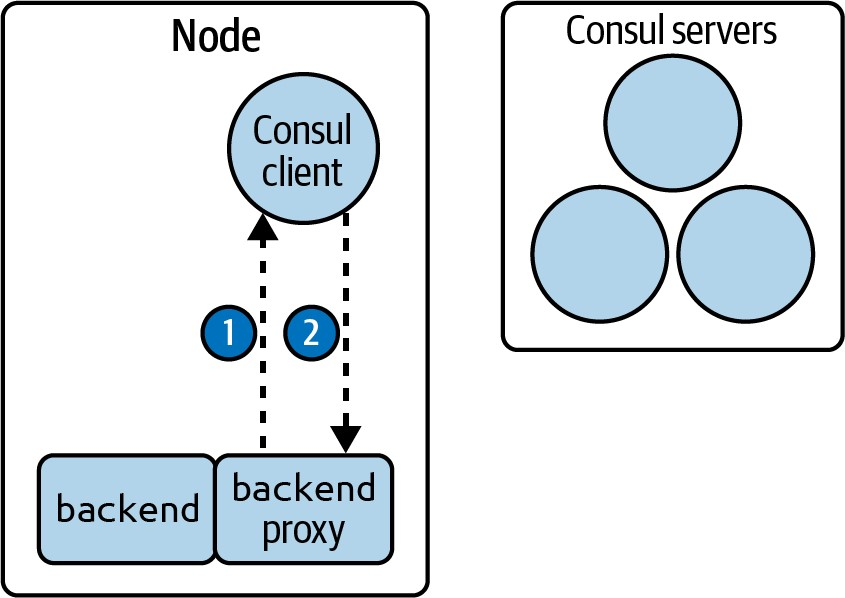
\includegraphics[width=0.7\linewidth]{Pics/example2}
		\caption{\label{fig:example2} Client Consul cấu hình proxy backend.}
		\label{fig:example2}
	\end{figure}
>>>>>>> Stashed changes
	
	\hspace{1.0cm}{Vault xác nhận và xác thực các đối tượng (người dùng, máy móc, ứng dụng) trước khi cung cấp cho chúng quyền truy cập vào các bí mật hoặc những dữ liệu lưu trữ nhạy cảm.\\}
	
<<<<<<< Updated upstream
	\begin{figure}[htp]	
=======
	\begin{figure}[h]
>>>>>>> Stashed changes
		\centering
		\includegraphics[width=0.7\textwidth]{"Pics/vault_interaction"}
		\caption{\label{fig:vault_interaction} Các cách giao tiếp giữa Vault và các đối tượng.}
		\label{fig:vault_interaction}
	\end{figure}
	
<<<<<<< Updated upstream
	\subsection{Kiến trúc của Vault}
	\hspace{1.0cm}{Vault là một hệ thống phức tạp với nhiều thành phần riêng biệt. Ở phần này chúng ta sẽ được hiểu chi tiết kiến trúc hệ thống của Vault và giúp chúng ta hiểu về Vault trong khi hiểu lý thuyết hoạt động.\\}
=======
	\hspace{0.3cm}{Proxy của giao diện người dùng cần biết địa chỉ của dịch vụ backend để thực hiện yêu cầu. Để thực hiện điều này, ứng dụng client Consul trên cùng một nút với dịch vụ giao diện người dùng sẽ xem danh mục máy chủ Consul để biết các phiên bản mới của dịch vụ backend (bước 1 trong Hình 2.10). Khi một phiên bản mới của dịch vụ backend được đăng ký vào danh mục, máy chủ Consul sẽ gửi địa chỉ mới đến ứng dụng client Consul (bước 2). Sau đó, máy client Consul cập nhật cấu hình proxy của dịch vụ giao diện người dùng với địa chỉ mới cho dịch vụ backend (bước 3).\\}
	
>>>>>>> Stashed changes
	\begin{figure}[h]
		\centering
		\includegraphics[width=1\textwidth]{"Pics/vault_architecture"}
		\caption{\label{fig:vault_architecture} Kiến trúc của Vault.}
		\label{fig:vault_architecture}
	\end{figure}
		
	\hspace{0.3cm}{Lớp mã hoá của Vault, hay còn được gọi là \textit{rào cản}, chịu trách nhiệm mã hoá và giải mã dữ liệu Vault. Khi máy chủ Vault được khởi động, nó bắt đầu viết dữ liệu vào Storage Backend. Vì Storage Backend nằm bên ngoài \textit{rào cản} nên nó được coi là không đáng tin cậy nên Vault sẽ mã hoá dữ liệu trước khi gửi chúng đến Storage Backend. Cơ chế này đảm bảo rằng nếu kẻ tấn công có mã độc dành quyền truy cập vào Storage Backend, thì dữ liệu sẽ không bị xâm phạm vì dữ liệu vẫn được mã hoá cho đến khi Vault giải mã dữ liệu. Storage Backend cung cấp một lớp dữ liệu bền được tích hợp liên tục, nơi dữ liệu được bảo mật và khả dụng mỗi khi khởi động lại máy chủ.\\}
	
	\hspace{0.3cm}{Khi máy chủ Vault được khởi động, máy chủ sẽ rơi vào trạng thái \textit{niêm phong}. Trước khi bất kì hoạt động nào đó được thực hiện bởi Vault, nó cần được ở trạng thái \textit{không niêm phong}. Bước này có thể thực hiện bằng cách cung cấp các khoá chưa niêm phong. Trong quá trình Vault khởi tạo, Vault sẽ tạo ra khoá mã hoá, thứ mà bảo vệ toàn bộ dữ liệu của Vault. Khoá này được bảo vệ bởi khoá gốc được lưu trữ cùng vói tất cả dữ liệu Vault khác, nhưng đuọc mã hoá bằng cơ chế khác: khoá chưa niêm phong.\\}
	
<<<<<<< Updated upstream
	\hspace{0.3cm}{Mặc định, Vault sử dụng \textbf{Shamir's Secret Sharing} để chia khoá chưa niêm phong thành một số phân đoạn được cấu hình (khoá chia sẻ hoặc khoá chưa niêm phong). Cần có một số lượng chính xác các phân đoạn để tái tạo khoá chưa niêm phong, sau đó khoá này được sử dụng để giải mã khoá gốc của Vault.\\}
	
	\begin{figure}[htp]
=======
	\begin{figure}[h]
		\centering
		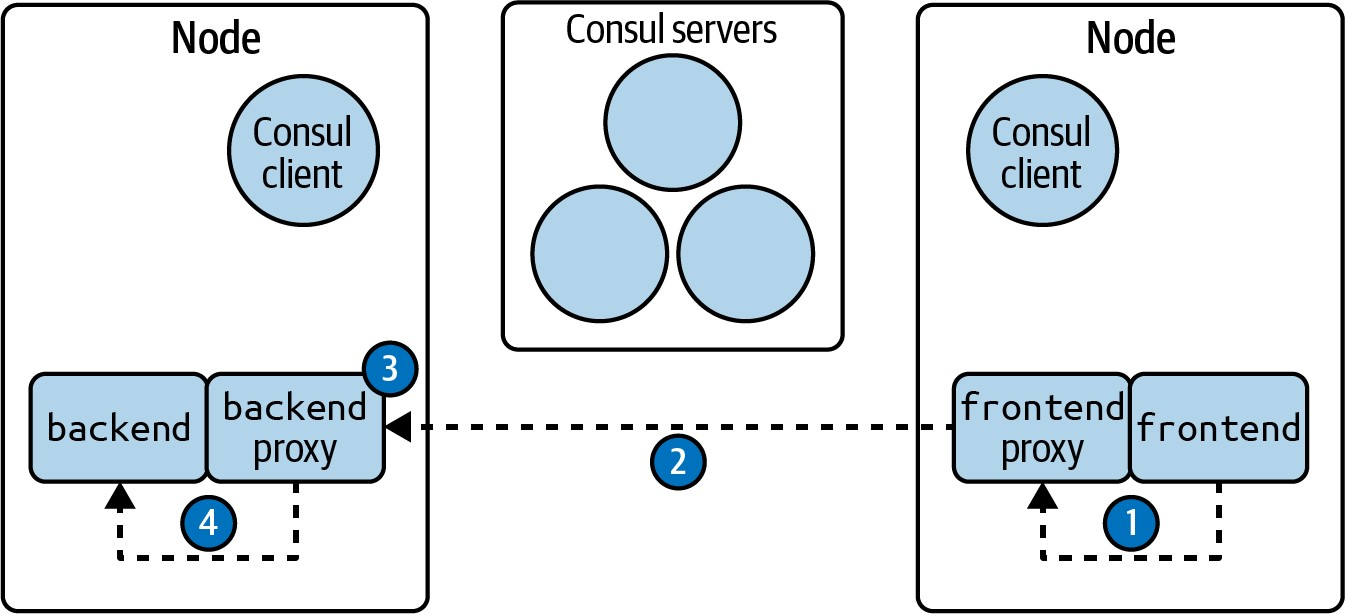
\includegraphics[width=0.7\linewidth]{Pics/example5}
		\caption{\label{fig:example5} Các proxy Sidecar ghi lại lưu lượng trong và ngoài và tuân theo các quy tắc được cấu hình của chúng để hành động trên lưu lượng đó.}
		\label{fig:example5}
	\end{figure}
	
	\hspace{0.3cm}{Ví dụ này minh họa cách máy chủ Consul, client và proxy sidecar hoạt động cùng nhau. Máy chủ Consul và client giao tiếp để chia sẻ dữ liệu về cụm và định cấu hình proxy sidecar. Các proxy Sidecar nắm bắt lưu lượng truy cập vào và ra và tuân theo các quy tắc được định cấu hình của chúng để hành động trên lưu lượng đó, chẳng hạn như bằng cách định tuyến nó tới một proxy khác hoặc không cho phép lưu lượng vì nó không được phép.}
	
	\subsection{Consul so với servece mesh khác}
	\hspace{1cm}{Có nhiều service mesh khác trên thị trường, chẳng hạn như Istio và Linkerd. Hầu hết các mắt service mesh đều tuân theo cùng một kiến trúc chung với một control plane quản lý các proxy sidecar. Consul là duy nhất trong số các mắt lưới khác ở chỗ control plane của nó có thể chạy hoàn toàn tách biệt với Kubernetes. Điều này có nghĩa là nếu bạn đang quản lý một cụm máy ảo thì bạn cũng không cần chạy Kubernetes.\\}
	
	\hspace{0.3cm}{Mỗi service mesh đều có ưu và nhược điểm tùy thuộc vào trường hợp sử dụng chính xác của bạn. Một cách tiếp cận tốt để chọn service mesh là tập trung vào ba trường hợp sử dụng hàng đầu của bạn, chẳng hạn như bảo mật, khả năng quan sát và hỗ trợ đa cụm, sau đó kiểm tra các service mesh phổ biến nhất và chọn một lưới mà bạn cảm thấy phù hợp nhất.}
	
	\subsection{Các tính năng khác của Consul}
	\hspace{1cm}{Consul không chỉ là một mạng service mesh. Đây cũng là kho lưu trữ khóa/giá trị cho cấu hình dịch vụ và giải pháp khám phá dịch vụ DNS. Khi sử dụng DNS, không có proxy sidecar. Các yêu cầu được định tuyến trực tiếp giữa các dịch vụ. Điều này có nghĩa là không có tính năng mã hóa, quan sát hoặc kiểm soát lưu lượng tự động.\\}
	
	\hspace{0.3cm}{Cuốn sách này tập trung vào các tính năng service mesh của Consul, nhưng bạn có thể truy cập tài liệu của Consul để tìm hiểu thêm về các tính năng khác của nó.}
	\section{Bảo mật trong Consul}
	\hspace{1cm}{Trong thế giới ngày nay, an ninh là tối quan trọng. Những kẻ tấn công tinh vi liên tục thăm dò các lỗ hổng có thể dẫn đến việc dữ liệu người dùng bị đánh cắp và hệ thống bị gián đoạn. Những cuộc tấn công này có thể hủy hoại danh tiếng của công ty và tiêu tốn hàng trăm nghìn đô la. Đồng thời, việc bảo vệ chống lại các cuộc tấn công này đang trở nên khó khăn hơn khi việc triển khai microservice ngày càng lớn và phức tạp hơn - do đó làm tăng mục tiêu tấn công của chúng.\\}
	
	\hspace{0.3cm}{Có nhiều khía cạnh để bảo mật hệ thống của bạn và mặc dù service mesh không thể giải quyết tất cả các khía cạnh đó nhưng nó đóng một vai trò quan trọng. Service mesh thực hiện các cải tiến bảo mật thông qua proxy sidecar chặn tất cả lưu lượng truy cập vào và ra khỏi dịch vụ. Một service mesh có thể cung cấp:}
	
	\begin{itemize}
		\item Mã hóa lưu lượng giữa các dịch vụ.
		\item Thực thi các quy tắc về dịch vụ nào có thể giao tiếp với nhau và loại yêu cầu nào được phép - ví dụ: đường dẫn HTTP nào có thể được truy cập.
		\item Một số giảm thiểu chống lại các cuộc tấn công từ chối dịch vụ bằng cách tăng độ tin cậy của dịch vụ.
	\end{itemize}

	\hspace{0.3cm}{Tuy nhiên, vì nó hoạt động ở cấp độ nền tảng nên service mesh không thể cung cấp:}
	
	\begin{itemize}
		\item Tự động vá các thư viện dễ bị tấn công.
		\item Loại bỏ các lỗi bảo mật trong mã code dịch vụ.
		\item Xác thực và ủy quyền người dùng (ví dụ: xác thực mật khẩu).
		\item Phát hiện xâm nhập (Phát hiện xâm nhập đang giám sát hoạt động đáng ngờ. Consul có thể giúp phát hiện xâm nhập vì nó cung cấp số liệu về các yêu cầu bị từ chối. Nếu một dịch vụ đột nhiên có nhiều yêu cầu bị từ chối, có khả năng kẻ tấn công đang cố truy cập dịch vụ đó).
		\item Các cải tiến bảo mật cấp dịch vụ khác.
	\end{itemize}

	\hspace{0.3cm}{Các cải tiến bảo mật mà service mesh cung cấp - mã hóa lưu lượng giữa các dịch vụ và thực thi các quy tắc về dịch vụ nào có thể giao tiếp với nhau - là một phần của việc triển khai mô hình bảo mật được gọi là zero trust network.\\}
	
	\hspace{0.3cm}{Phần này bắt đầu với phần mô tả về mô hình zero trust network và lý do tại sao nó là một cải tiến so với mô hình cũ hơn. Sau đó, trình bày cách Consul triển khai zero trust network và mô tả mã hóa TLS.}
	\subsection{Zero trust network trong Consul}
	\hspace{1cm}{Kiến trúc an ninh mạng truyền thống là theo mô hình castle and moat. Trong mô hình castle and moat, các dịch vụ được triển khai trong một mạng riêng nội bộ (castle - lâu đài) không được kết nối với internet công cộng. Tường lửa (moat - hào nước) bảo vệ quyền truy cập vào mạng nội bộ (Tường lửa là phần mềm hoặc phần cứng kiểm soát quyền truy cập ở rìa mạng - nơi các hệ thống được kết nối với cả mạng riêng và mạng công cộng). Bộ cân bằng tải được triển khai bên ngoài mạng riêng và được phép truy cập thông qua tường lửa. Vì tường lửa đã được đặt sẵn, giả định rằng mọi thứ chạy bên trong mạng nội bộ đều có thể tin cậy được. Vì lý do này, không cần mã hóa, xác thực hoặc ủy quyền giữa các dịch vụ nội bộ.\\}
	
	\begin{figure}[h]
		\centering
		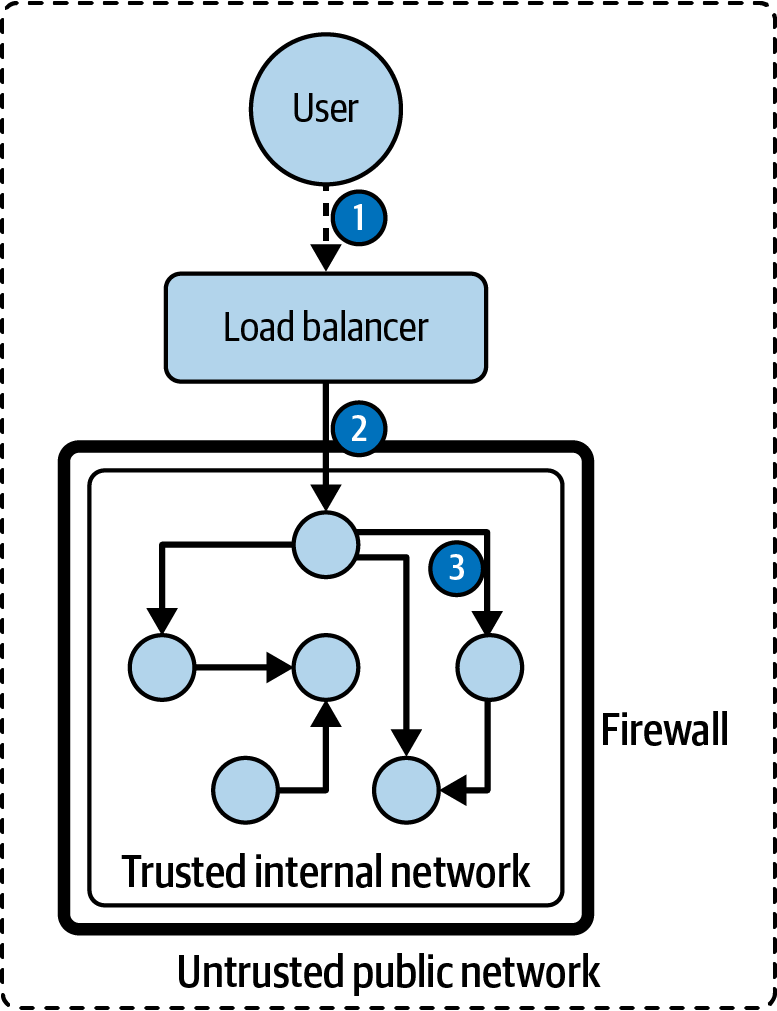
\includegraphics[width=0.5\linewidth]{Pics/castle_and_moat_modal}
		\caption{\label{fig:castleandmoatmodal} Định tuyến bên trong kiến trúc castle and moat.}
		\label{fig:castleandmoatmodal}
	\end{figure}
	
	\hspace{0.3cm}{Hình 2.12 cho thấy lưu lượng truy cập được định tuyến như thế nào qua kiến trúc castle and moat. Ở bước 1, yêu cầu của người dùng được chuyển đến bộ cân bằng tải. Bộ cân bằng tải chuyển tiếp yêu cầu qua tường lửa tới một dịch vụ đang chạy trong mạng nội bộ đáng tin cậy (bước 2). Dịch vụ đó thực hiện cuộc gọi đến các dịch vụ upstream của nó (bước 3). Các cuộc gọi này không được mã hóa và các dịch vụ upstream không kiểm tra ủy quyền vì các cuộc gọi đến từ bên trong mạng nội bộ đáng tin cậy.\\}
	
	\hspace{0.3cm}{Vấn đề với mô hình castle and moat là những kẻ tấn công giành được quyền truy cập vào toàn bộ hệ thống nếu chúng xâm phạm bất kỳ điểm nào trong mạng nội bộ, như trong Hình 2.13. Điều này có nghĩa là bảo mật của hệ thống chỉ tốt bằng liên kết yếu nhất của nó.\\}
	
	\begin{figure}[h]
		\centering
		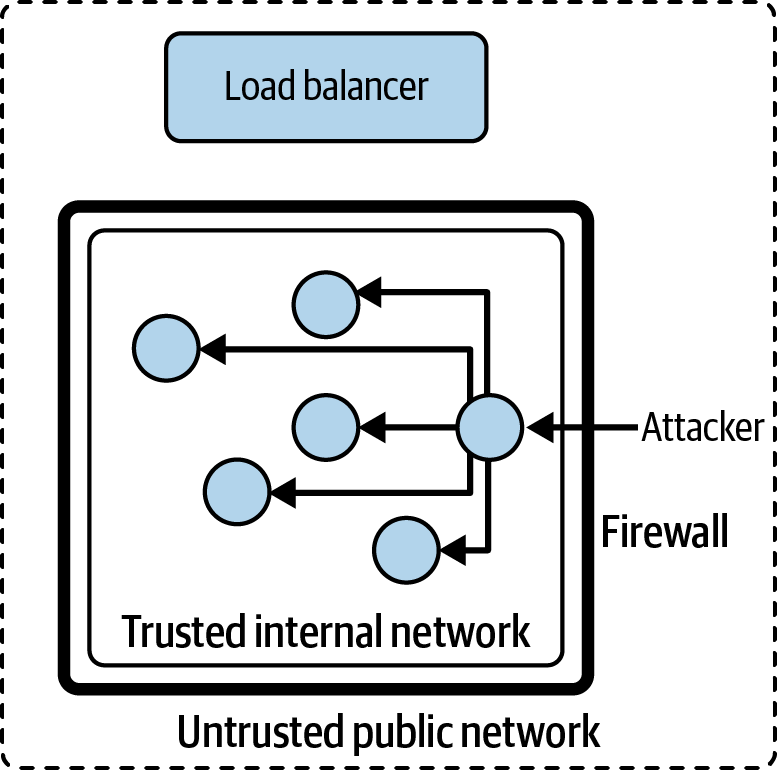
\includegraphics[width=0.5\linewidth]{Pics/threat_of_castle_and_moat}
		\caption{\label{fig:threatofcastleandmoat} Trong kiến trúc castle and moat, nếu kẻ tấn công xâm phạm một dịch vụ, chúng có thể yêu cầu tất cả các dịch vụ và cơ sở dữ liệu bên trong mạng.}
		\label{fig:threatofcastleandmoat}
	\end{figure}
	
	\hspace{0.3cm}{Đây không phải là một điểm yếu lý thuyết. Vào năm 2015, tin tặc đã đánh cắp hàng triệu hồ sơ nhạy cảm về nhân viên chính phủ từ Văn phòng Quản lý Nhân sự Hoa Kỳ (OPM). Những kẻ tấn công đã giành được quyền truy cập bằng cách xâm nhập vào hệ thống của một công ty hợp đồng có máy chủ có toàn quyền truy cập vào mạng OPM. Từ đó, họ có thể tự do trích xuất dữ liệu từ các máy chủ OPM.\\}
	
	\hspace{0.3cm}{Điểm yếu của hệ thống castle and moat là không thể chấp nhận được đối với hầu hết các công ty, vì vậy các kỹ sư bảo mật đề xuất một mô hình khác: zero trust network.\\}
	
	\hspace{0.3cm}{Trong zero trust network, bạn cho rằng mạng nội bộ bị xâm phạm. Do đó, các dịch vụ không hoàn toàn tin tưởng các yêu cầu đơn giản chỉ vì chúng đến từ bên trong mạng nội bộ. Thay vào đó, các dịch vụ thực hiện mã hóa, xác thực và ủy quyền cho tất cả các yêu cầu.}
	
	\subsubsection{Mã hóa}
	\hspace{1cm}{Quá trình sửa đổi dữ liệu sao cho bên thứ ba không thể đọc dữ liệu gốc chưa sửa đổi, nhưng người nhận thì có thể. Trong mạng máy tính, quy trình mã hóa TLS thường được sử dụng để đảm bảo rằng các bên thứ ba không thể chặn và đọc dữ liệu được gửi giữa người dùng và trang web mà họ đang xem. TLS được sử dụng bí mật khi bạn truy cập các trang web https://.}
	
	\subsubsection{Xác thực}
	\hspace{1cm}{Quá trình xác thực rằng một thực thể là người đã được xác minh, công nhận. Ví dụ: nếu người dùng tuyên bố là người dùng quản trị, thì xác thực là quá trình kiểm tra xem mật khẩu họ cung cấp có khớp với mật khẩu dự kiến hay không. Sau khi một thực thể được xác thực, bạn vẫn cần kiểm tra xem họ có được phép thực hiện hành động mà họ đang cố thực hiện hay không.}
	
	\subsubsection{Ủy quyền}
	\hspace{1cm}{Quá trình xác thực rằng một thực thể được xác thực được phép thực hiện một hành động cụ thể nào đó hay không. Ví dụ: người dùng đã đăng nhập có thể được xác thực nhưng có lẽ họ không được phép xem bảng quản trị.}

	\subsection{Mã hóa trong Consul}
	\hspace{1cm}{Mã hóa là cần thiết trong mạng zero trust network vì dịch vụ bị xâm phạm có thể đọc lưu lượng được truyền giữa các dịch vụ khác- điều này được gọi là traffic sniffng hoặc tấn công trung gian (xem Hình 2.14). (Có nhiều cơ chế để một dịch vụ bị xâm nhập chặn bắt lưu lượng truy cập. Nếu dịch vụ bị xâm nhập nằm trên cùng một node với một dịch vụ khác, dịch vụ đó có thể có quyền kiểm tra lưu lượng mạng của các quy trình khác. Hoặc một dịch vụ bị xâm phạm có thể sử dụng một kỹ thuật gọi là giả mạo Giao thức phân giải địa chỉ (ARP) để khiến một dịch vụ khác gửi nhầm lưu lượng truy cập của nó đến dịch vụ bị xâm phạm thay vì đích dự kiến).\\}
	
	\begin{figure}[h]
		\centering
		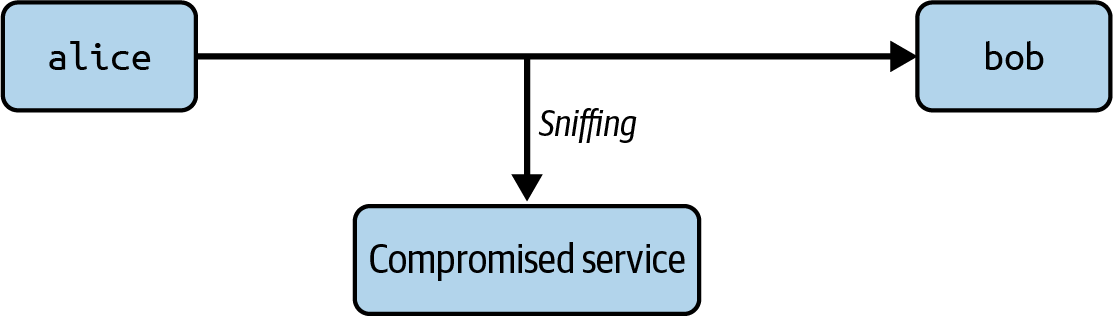
\includegraphics[width=0.7\linewidth]{Pics/sniffing}
		\caption{\label{fig:sniffing} Một dịch vụ bị xâm nhập có thể chặn truy tìm được gửi giữa hai dịch vụ khác.}
		\label{fig:sniffing}
	\end{figure}
	
	\hspace{0.3cm}{Mã hóa ngăn chặn các cuộc tấn công trung gian vì những kẻ tấn công không thể đọc dữ liệu được gửi giữa hai dịch vụ. Chỉ dịch vụ đích mới có thể giải mã dữ liệu. Như thể hiện trong Hình 2.13, nếu Bob là dịch vụ duy nhất có khả năng giải mã lưu lượng truy cập từ dịch vụ Alice, thì việc kẻ tấn công chặn lưu lượng cũng không thành vấn đề.\\}
	
	\begin{figure}[h]
		\centering
		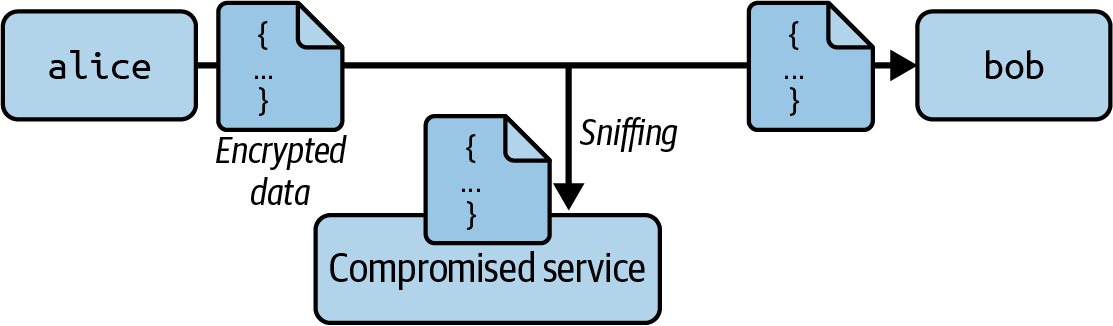
\includegraphics[width=0.7\linewidth]{Pics/encrypt_prevent_sniffing}
		\caption{\label{fig:encryptpreventsniffing} Dữ liệu điện tử hiện đã được mã hóa, do đó, ngay cả khi dịch vụ bị xâm phạm sniffing, chúng cũng không thể lấy được nội dung gốc.}
		\label{fig:encryptpreventsniffing}
	\end{figure}
	
	\hspace{0.3cm}{Consul sử dụng mã hóa TLS để mã hóa lưu lượng giữa các dịch vụ.}
	
	\subsubsection{Mã hóa TLS}
	\hspace{1cm}{Mã hóa TLS có ba bước (xem Hình 2.16 để biết minh họa):}
	\begin{enumerate}
	\item Dịch vụ nguồn và đích đồng ý về khóa mã hóa.
	\item Dịch vụ nguồn mã hóa tin nhắn của nó bằng khóa đã thỏa thuận và gửi tin nhắn được mã hóa đến dịch vụ đích.
	\item Dịch vụ đích giải mã tin nhắn bằng khóa đã thỏa thuận.
	\end{enumerate}

	\begin{figure}[h]
		\centering
		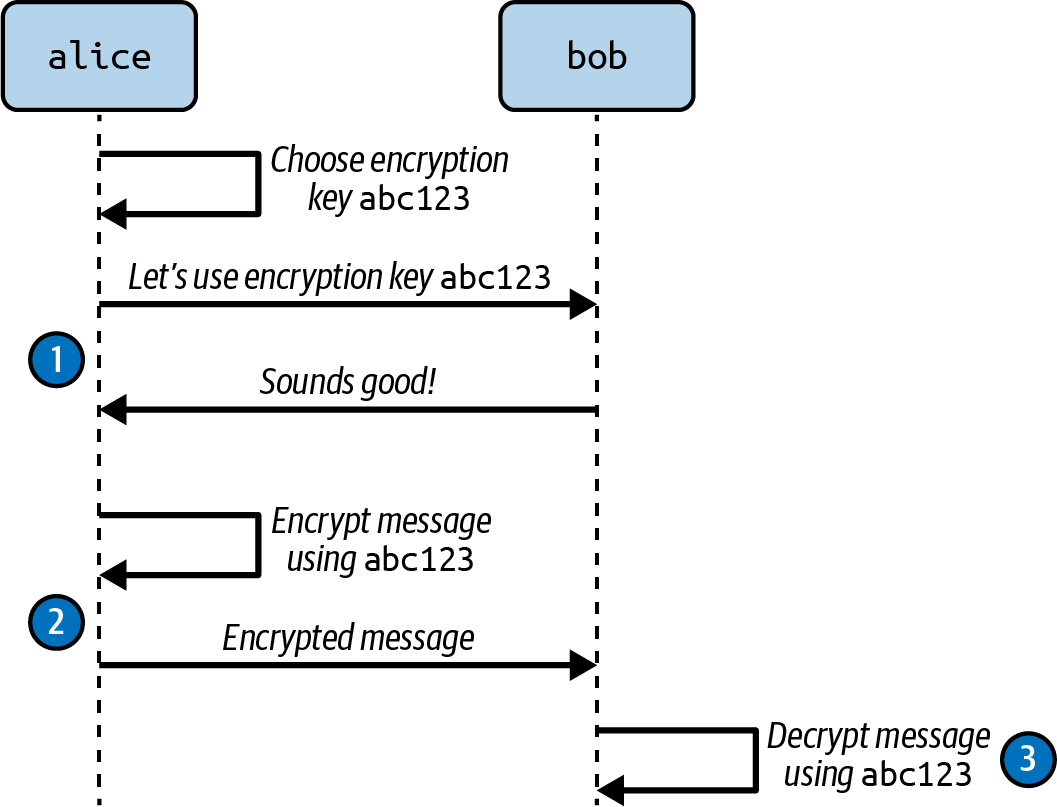
\includegraphics[width=0.7\linewidth]{Pics/TLS}
		\caption{\label{fig:tls} Một minh họa về mã hóa TLS.}
		\label{fig:tls}
	\end{figure}
	
	\hspace{0.3cm}{Miễn là những kẻ tấn công trung gian không biết khóa mã hóa, chúng không thể giải mã tin nhắn. Loại mã hóa này được gọi là mã hóa đối xứng vì cả hai bên đều biết khóa mã hóa.\\}
	
	\hspace{0.3cm}{Nhưng làm thế nào để khóa mã hóa đối xứng được thỏa thuận mà không có kẻ tấn công chặn nó? Đây là lúc mật mã khóa công khai phát huy tác dụng.\\}
	
	\hspace{0.3cm}{Mật mã khóa công khai là một phương pháp mã hóa sử dụng các cặp khóa: khóa bí mật và khóa công khai. Các khóa được liên kết về mặt toán học sao cho các thông báo được mã hóa bằng khóa công khai chỉ có thể được giải mã bằng khóa bí mật. Mật mã khóa công khai cho phép cả hai dịch vụ đồng ý với khóa mã hóa đối xứng mà khóa đó không được gửi qua mạng, nơi khóa có thể bị đánh cắp.\\}
	
	\hspace{0.3cm}{Hãy xem qua một ví dụ sử dụng hai dịch vụ tưởng tượng, Alice và Bob, muốn đồng ý về một khóa mã hóa đối xứng:}
	
	\begin{enumerate}
	\item Dịch vụ Alice tạo hai khóa, một khóa bí mật có tên alice-priv và một khóa công khai có tên alice-pub.
	\item Dịch vụ Alice gửi khóa công khai của nó - alice-pub đến dịch vụ Bob. Khóa được gửi dưới dạng văn bản rõ để kẻ tấn công có thể nhìn thấy khóa.
	\item Dịch vụ Bob cũng làm như vậy. Nó tạo ra hai khóa, bob-priv và bob-pub, đồng thời gửi khóa bob-pub cho Alice. Một lần nữa, kẻ tấn công có thể thấy khóa bob-pub.
	\item Ngay bây giờ Alice sẵn sàng gửi khóa mã hóa đối xứng cho Bob. Alice mã hóa khóa mã hóa đối xứng bằng khóa công khai của Bob - bob-pub.
	\item Alice gửi thông điệp được mã hóa này cho Bob. Một lần nữa, kẻ tấn công có thể nhìn thấy thông điệp được mã hóa này, nhưng điều kỳ diệu của mật mã khóa công khai là kẻ tấn công không thể giải mã thông điệp bằng các khóa công khai alice-pub hoặc bob-pub. Thuật toán sử dụng để mã hóa thông điệp được thiết kế sao cho chỉ khóa bí mật của Bob (bob-priv) mới có thể giải mã nó.
	\item Bob nhận được thông điệp được mã hóa và sử dụng khóa riêng của nó - bob-priv để giải mã.
	\item Giờ đây, khóa mã hóa đối xứng đã được thỏa thuận một cách an toàn, Alice và Bob có thể tự do gửi thêm thông điệp bằng cách mã hóa chúng khóa mã hóa đối xứng.
	\end{enumerate}

	\begin{figure}[h]
		\centering
		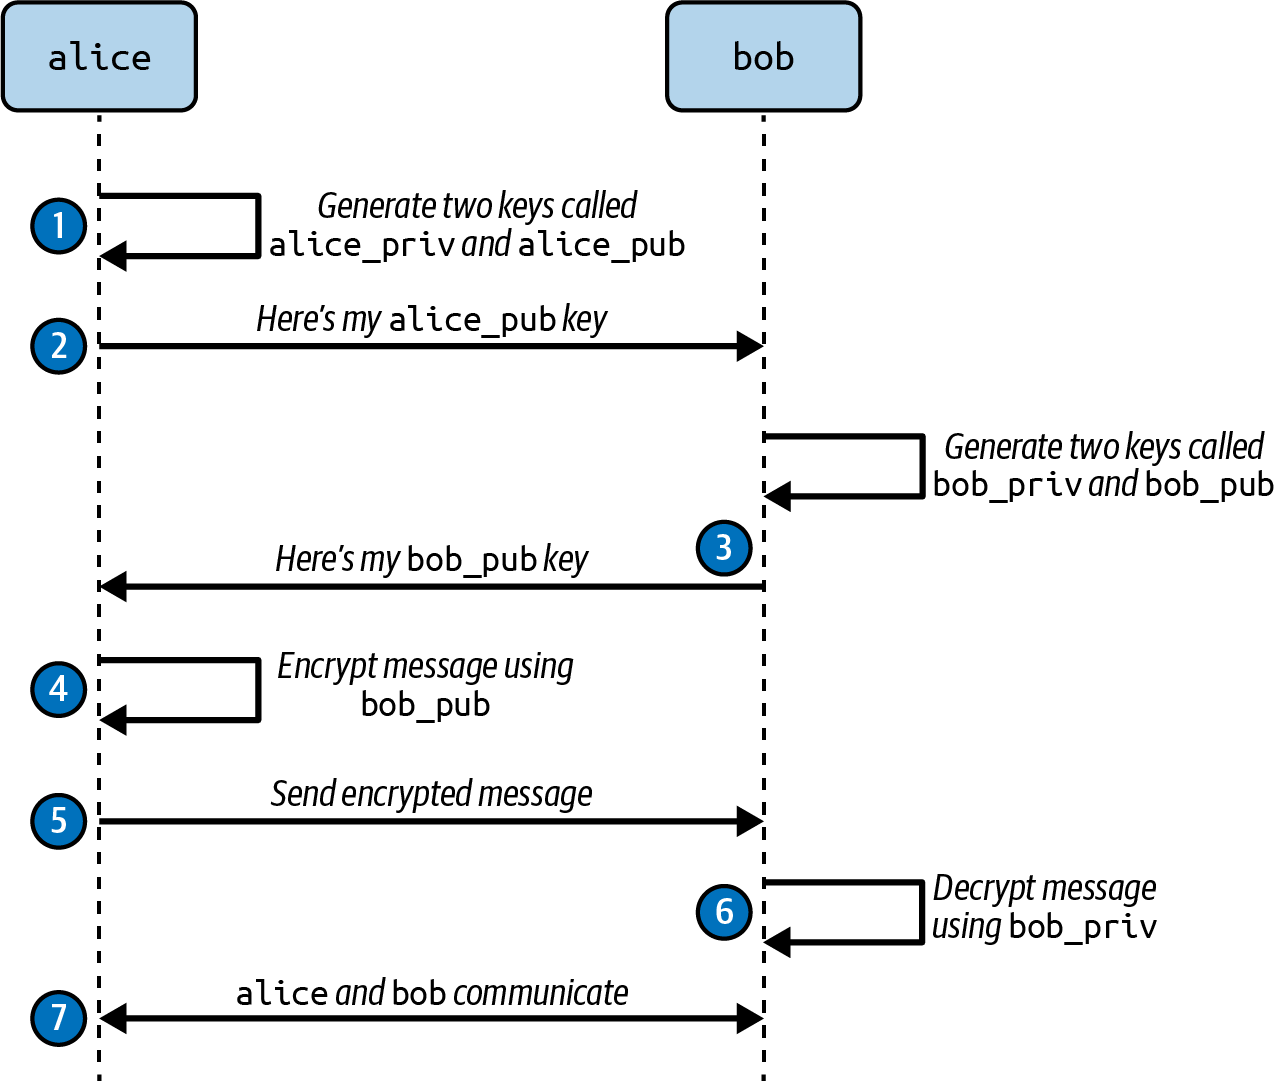
\includegraphics[width=0.7\linewidth]{Pics/public-key_cryptography}
		\caption{\label{fig:public-keycryptography} Sơ đồ mật mã khóa công khai.}
		\label{fig:public-keycryptography}
	\end{figure}
	
	\hspace{0.3cm}{Vì lý do hiệu suất, mật mã khóa công khai chỉ được sử dụng khi bắt đầu kết nối TLS để đồng ý một cách an toàn về khóa mã hóa đối xứng. Từ đó trở đi, khóa mã hóa đối xứng đó được sử dụng để mã hóa tất cả dữ liệu được gửi giữa hai dịch vụ.\\}
	
	\hspace{0.3cm}{Đó chính là cách hoạt động của mã hóa TLS, Consul sử dụng TLS để mã hóa lưu lượng service mesh.}
	
	\subsubsection{Mã hóa trong Consul}
	\hspace{1cm}{Mã hóa TLS trong Consul được bật theo mặc định. Khi một dịch vụ đưa ra yêu cầu thông qua proxy sidecar của nó, proxy sẽ tự động mã hóa yêu cầu đó bằng TLS. Dịch vụ có thể tiếp tục thực hiện các yêu cầu không được mã hóa và proxy đảm bảo các yêu cầu đó được mã hóa trước khi chúng rời khỏi mạng cục bộ.\\}
	
	\hspace{0.3cm}{Quá trình này được thể hiện trong Hình 2.18. Ở bước 1, Consul cung cấp khóa công khai và khóa bí mật cho từng proxy. Khi giao diện người dùng gửi một yêu cầu không được mã hóa đến chương trình backend, thì yêu cầu đó sẽ bị chặn bởi proxy của giao diện người dùng (bước 2) và mã hóa yêu cầu đó trước khi chuyển tiếp đến chương trình backend (bước 3). Ở phía bên nhận, proxy của chương trình backend sẽ chặn yêu cầu (bước 4) và giải mã nó trước khi chuyển tiếp đến dịch vụ đích (bước 5).\\}
	
	\begin{figure}
		\centering
		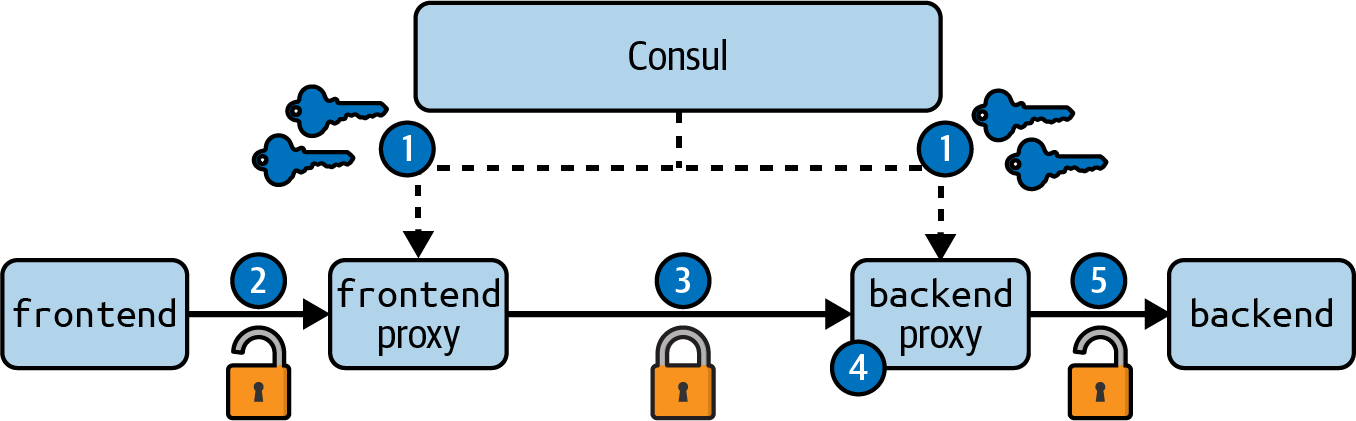
\includegraphics[width=0.7\linewidth]{Pics/Sidecar_proxies_automatically_encrypt}
		\caption{\label{fig:sidecarproxiesautomaticallyencrypt} Sidecar proxy tự động mã hóa lưu lượng bằng TLS.}
		\label{fig:sidecarproxiesautomaticallyencrypt}
	\end{figure}
	
	\hspace{0.3cm}{Với cơ chế này, các dịch vụ không cần phải sửa đổi để sử dụng TLS - tất cả đều diễn ra tự động mà chúng không hề hay biết.\\}
	
	\hspace{0.3cm}{Đó chính xác là cách Consul thực hiện mã hóa. Mã hóa là điều cần thiết trong một zero trust network, nhưng nó vẫn không đủ. Nếu không có xác thực và ủy quyền, một dịch vụ bị xâm phạm vẫn có thể thực hiện các yêu cầu thông qua proxy sidecar của nó tới bất kỳ dịch vụ nào trong mạng.}
	
	\subsection{Xác thực trong Consul}
	\hspace{1cm}{Xác thực là quá trình xác minh rằng ai đó là người mà đã được xác minh; đó là về việc xác minh danh tính. Trong mạng dịch vụ, điều này có hai phần: dịch vụ nguồn phải xác minh rằng dịch vụ đích thực sự là dịch vụ mà nó muốn giao tiếp và dịch vụ đích phải xác minh rằng dịch vụ nguồn thực sự là dịch vụ mà nó yêu cầu.\\}
	
	\hspace{0.3cm}{Cụ thể, nếu giao diện người dùng đang gọi phần backend, thì giao diện người dùng cần đảm bảo rằng nó thực sự đang nói chuyện với phần backend. Nếu nó không kiểm tra, thì nó có thể đang gửi yêu cầu của mình tới kẻ tấn công. Backend cũng cần xác minh dịch vụ nào đang thực hiện yêu cầu để có thể kiểm tra xem dịch vụ đó có được phép giao tiếp với nó hay không.\\}
	
	\hspace{0.3cm}{Consul cũng tận dụng TLS để thực hiện xác thực. Khi các dịch vụ trao đổi khóa công khai của họ, họ thực sự trao đổi chứng chỉ. Chứng chỉ này chứa khóa công khai và thông tin về dịch vụ, chẳng hạn như ID của nó.\\}
	
	\hspace{0.3cm}{Đây là các bước liên quan đến xác thực TLS (xem Hình 2.19 để minh họa):}
	
	\begin{enumerate}
	\item Consul cấp chứng chỉ công khai và khóa bí mật cho từng dịch vụ. Được mã hóa trong chứng chỉ công khai là ID của dịch vụ đó.
	\item Trong quá trình trao đổi khóa, chứng chỉ công khai cho mỗi dịch vụ được trao đổi.
	\item Mỗi dịch vụ kiểm tra chứng chỉ công khai của dịch vụ kia và đảm bảo rằng ID dịch vụ là những gì được mong đợi. Ví dụ: dịch vụ giao diện người dùng sẽ xác minh rằng chứng chỉ dành cho dịch vụ backend và dịch vụ backend sẽ xác minh rằng chứng chỉ dành cho dịch vụ giao diện người dùng.
	\item Nếu danh tính được xác minh, yêu cầu sẽ tiếp tục.
	\end{enumerate}

	\begin{figure}[h]
		\centering
		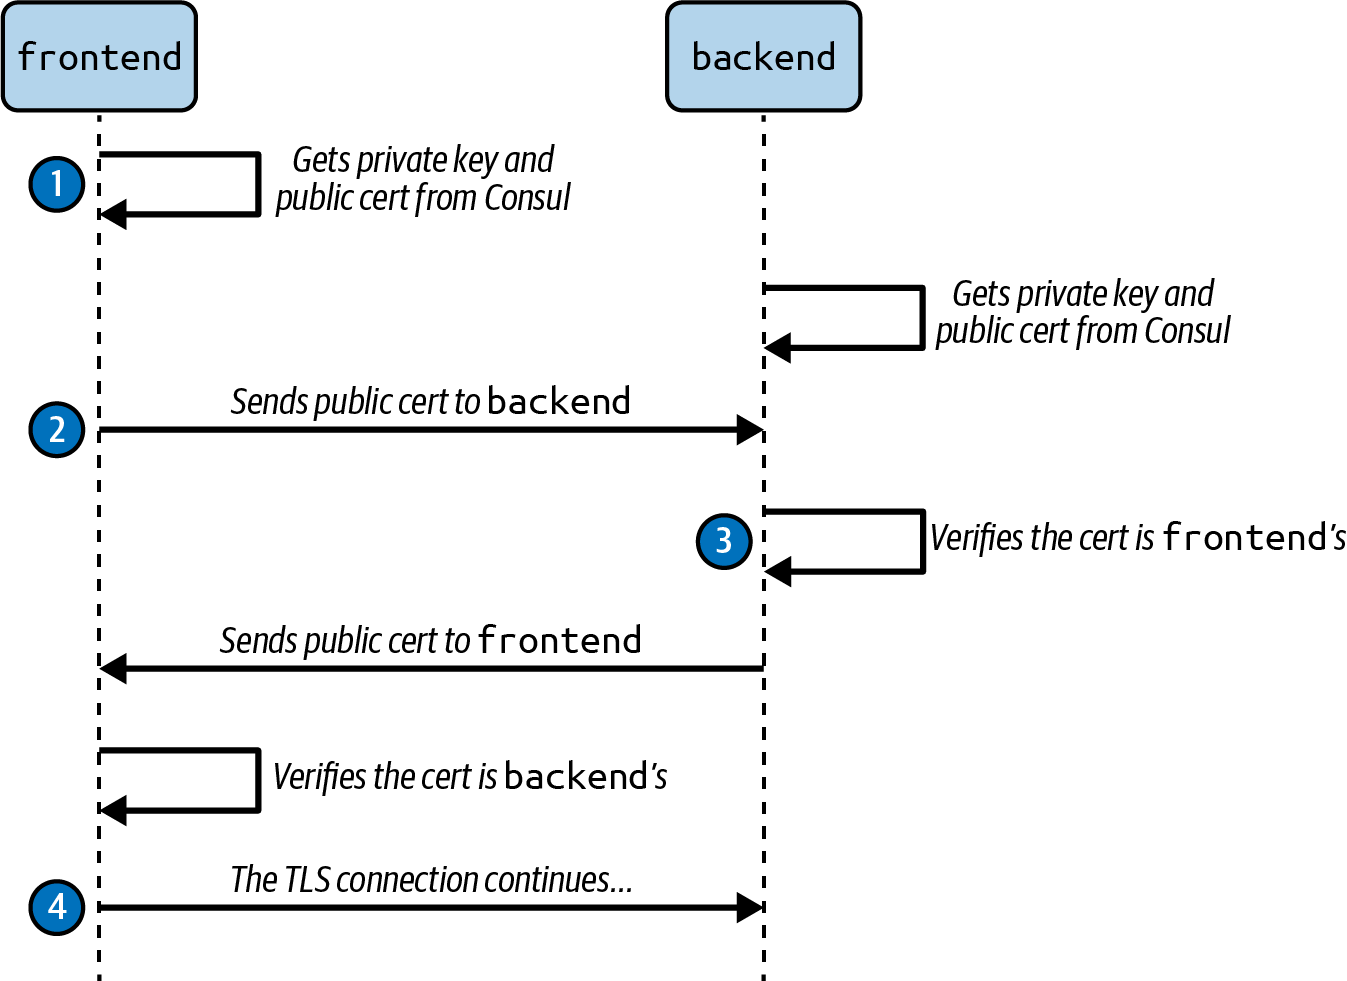
\includegraphics[width=0.7\linewidth]{Pics/TLS_provide_authentication}
		\caption{\label{fig:tlsprovideauthentication} TLS được sử dụng để cung cấp xác thực.}
		\label{fig:tlsprovideauthentication}
	\end{figure}
	
	\hspace{0.3cm}{Chúng ta có thể tự hỏi điều gì ngăn kẻ tấn công tạo chứng chỉ công khai của riêng chúng để mạo danh bất kỳ dịch vụ nào. Để ngăn chặn điều này, Consul hoạt động như một cơ quan cấp chứng chỉ.\\}
	
	\hspace{0.3cm}{Cơ quan cấp chứng chỉ là một thực thể cấp chứng chỉ được ký bằng mật mã sao cho chúng chỉ có thể đến từ cơ quan cấp chứng chỉ đó. Cơ quan cấp chứng chỉ cũng có chứng chỉ công khai được gọi là chứng chỉ của cơ quan cấp chứng chỉ (chứng chỉ CA). Khi xuất trình chứng chỉ công khai của dịch vụ - ví dụ: chứng chỉ backend - bên thứ ba có thể sử dụng chứng chỉ CA để kiểm tra xem chứng chỉ công khai có được ký bởi cơ quan cấp chứng chỉ đó hay không.\\}
	
	\hspace{0.3cm}{Cụ thể, ngoài chứng chỉ công khai và khóa bí mật mà Consul cấp cho từng dịch vụ, Consul còn cấp cho từng dịch vụ chứng chỉ CA của mình. Sau đó, chứng chỉ CA này có thể được sử dụng để xác minh rằng Consul thực sự đã cấp chứng chỉ công khai và việc tin cậy ID dịch vụ được mã hóa bên trong là an toàn.\\}
	
	\begin{figure}[h]
		\centering
		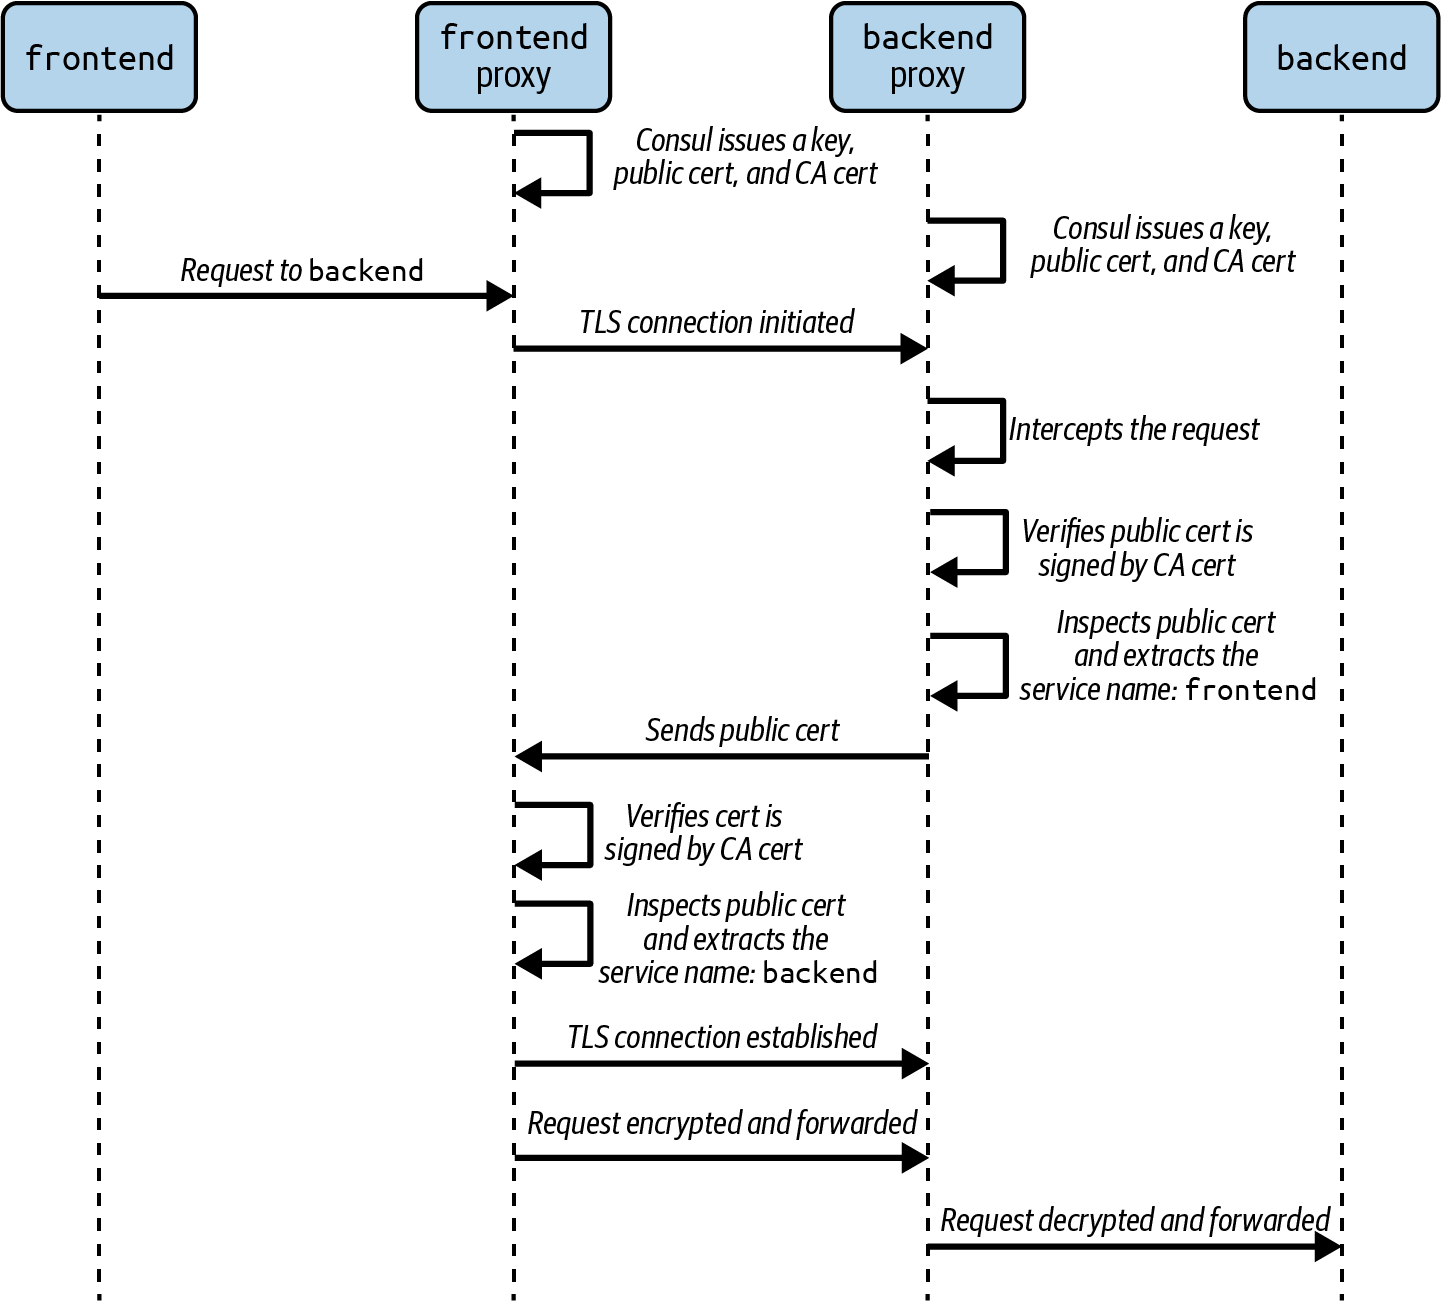
\includegraphics[width=0.7\linewidth]{Pics/frontend_talk_to_backend_securely}
		\caption{\label{fig:frontendtalktobackendsecurely} Quy trình khi giao diện người dùng giao tiếp với phần backend một cách an toàn.}
		\label{fig:frontendtalktobackendsecurely}
	\end{figure}
	
	\hspace{0.3cm}{Bạn có thể xem các chứng chỉ công khai của từng dịch vụ bằng công cụ openssl.}
	\subsection{Ủy quyền trong Consul}
	\hspace{1cm}{Ủy quyền là quá trình xác định xem một thực thể được xác thực có được phép thực hiện một hành động nhất định hay không. Ví dụ: dịch vụ này có được phép thực hiện các yêu cầu đối với dịch vụ đó hay được phép truy cập vào một đường dẫn HTTP cụ thể không?\\}
	
	\hspace{0.3cm}{Consul thực hiện ủy quyền thông qua hệ thống chủ đích của nó. Chủ đích là các quy tắc chi phối các dịch vụ nào được phép giao tiếp.\\}
	
	\hspace{0.3cm}{Mọi chủ đích đều có nguồn gốc và đích đến. Ví dụ: một chủ đích có thể cho phép một giao diện người dùng dịch vụ cụ thể (nguồn) kết nối với một dịch vụ backend cụ thể (đích). Ngoài ra, ký tự đại diện có thể được sử dụng làm nguồn hoặc đích, chẳng hạn như cho phép một cổng vào kết nối với bất kỳ dịch vụ nào hoặc bất kỳ dịch vụ nào kết nối với bất kỳ dịch vụ nào khác.\\}
	
	\hspace{0.3cm}{Ngoài việc chỉ định các quy tắc dựa trên dịch vụ nguồn và đích, bạn có thể sử dụng các chủ đích để kiểm soát các phương thức, đường dẫn và tiêu đề HTTP hoặc gRPC nào được ủy quyền. Consul gọi những chủ đích này là nhận biết ứng dụng vì chúng liên quan đến cách ứng dụng thực sự hoạt động. Ví dụ: bạn có thể tạo một chủ đích cho phép cổng vào truy cập vào bất kỳ đường dẫn nào trên dịch vụ giao diện người dùng ngoại trừ /admin.\\}
	
	\hspace{0.3cm}{Cơ chế thực thi chủ đích như sau:}
	
	\begin{enumerate}
	\item Dịch vụ nguồn gửi yêu cầu đến dịch vụ đích.
	\item Proxy của dịch vụ đích xác minh chứng chỉ công khai của dịch vụ nguồn và trích xuất tên dịch vụ từ ID.
	\item Proxy của dịch vụ đích kiểm tra danh sách các chủ đích của nó để đảm bảo rằng dịch vụ nguồn được phép thực hiện kết nối.
	\item Nếu đã đặt chủ đích nhận biết ứng dụng, proxy của dịch vụ đích cũng xác minh rằng yêu cầu cụ thể đó được cho phép.
	\end{enumerate}

	\chapter{Triển khai Consul trên Kubernetes}
	\section{Mô hình triển khai}
	\section{Các bước triển khai Consul trên Kubernetes}
	\section{Thực nghiệm}
	\subsection{Kịch bản một: Mã hoá và thiết lập luật đường truyền giữa các micorserivce trong kubernetes}
	\subsubsection{Mô hình kịch bản}
	 \begin{figure}[h]
>>>>>>> Stashed changes
		\centering
		\includegraphics[width=1\textwidth]{"Pics/shamir_secret_sharing"}
		\caption{\label{fig:shamir_secret_sharing} Cách thức chia khoá của Vault.}
		\label{fig:shamir_secret_sharing}
	\end{figure}

	\hspace{0.3cm}{Cả số lượng chia sẻ và số lượng phân đoạn tối thiểu đều có thể tuỳ chỉnh. Kỹ thuật của Shamir có thể bị vô hiệu hoá và khoá gốc có thể được sử dụng trực tiếp để mở khoá. Sau khi Vault truy xuất khoá mã hoá, nó sẽ giải mã dữ liệu trong phần Storage Backend và chuyển sang trạng thái không được niêm phong. Sau khi được huỷ niêm phong, Vault tải các thiết bị kiểm tra đã được cấu hình, phương thức xác thực và công cụ bảo mật.\\}
	
	\hspace{0.3cm}{Cấu hình của thiết bị kiểm tra, phương pháp xác thực và công cụ bảo mật nhạy cảm về bảo mật và được lưu trong Vault. Các người dùng với quyền được chỉnh sửa chúng và không thể chỉ định bên ngoài rào cản. bằng cách lwu trữ chúng trong Vault, các thay đổi được hệ thống ACL(Access Control List) bảo vệ và theo dõi bằng nhật ký kiểm tra.\\}
	
	\hspace{0.3cm}{Các yêu cầu có thể được xử lý từ API HTTP đến lõi sau khi Vault được huỷ niêm phong. Lõi quản lý luồng yêu cầu thông qua hệ thống, thực thi ACL và đảm bảo việc ghi nhật kí kiểm tra được thực hiện.\\}
	
	\hspace{0.3cm}{Khi máy khách kết nối lần đầu voiws Vault, máy khác đó cần được xác thực. Vault cung cấp phương thức xác thực có thể cấu hình và cung cấp tính linh hoạt trong cơ chế xác thực được sử dụng. Các cơ chế như tên người dùng/mật khẩu hoặc GitHub có thể được sử dụng cho người vận hành, trong khi các ứng dụng có thể sử dụng khoá công khai/bí mật hoặc mã để xác thực. Yêu cầu xác thực được truyền qua lõi và vào phương thức xác định yêu cầu có hợp lệ hay khôn và trả về các chính xác liên quan.\\}
	
	\hspace{0.3cm}{Chính sách chỉ là một quy tắc ACL được đặt tên. Ví dụ: Chính xác "root" được tính hợp sẵn và cho phép truy cập vào tất cả các tài nguyên. Bạn có thể tạo bất kỳ số lượng chính sách được đặt tên nào với quyền kiểm soát chi tiết với các đường dẫn. Vault hoạt động ở chế độ được phép truy cập, nghĩa là hành động được phép trừ khi quyền truy cập được cấp thông qua chính sách một cách rõ ràng. Vì người dùng có thể có nhiều chính sách được liên kết, các hành động được phép thực hiện khi chính sách cho phép. Các chính sách được lưu trữ và quản lý bởi một kho chính sách nội bộ. Kho chính sách nội bộ này bị ảnh hưởng thông qua Backend Storage, luôn được gắn tại \textit{sys/}. \\}
	
	\hspace{0.3cm}{Sau khi quá trình xác thực diễn ra và phương thức xác thực cung cấp một tập hợp các chính sách áp dụng, một client token được tạo ra và quản lý bởi kho lưu trữ. Client token sẽ được sử dụng để thực hiện các yêu cầu trong tương lại. Phương thức client token này tương tự như cookie do trang web gửi khi người dùng đăng nhập. Tuỳ thuộc vào cấu hình phương thức xác thực, client token có thể có thời hạn liên kết với nó, và nó thể cần phải được gia hạn định kỳ để tránh mất hiệu lực.\\}

	
	\hspace{0.3cm}{Sau khi được xác thực, yêu cầu được thực hiện bằng cách cung cấp Client token. Client token được sử dụng để xác thực máy khách, đảm bảo rằng nó được xác thực trong khi tải các chính sách liên quan. Các chính sách được sử dụng để xác thực yêu cầu của máy khách. Các yêu cầu sau đó được hướng tới secret engine, thứ mà được xử lý tuỳ thuộc vào loại của nó. Khi mà các secret engine trả lại các secret, lõi sẽ đăng kí nó với trình quản lý hết hạn và đính kèm nó với ID cho hợp đồng. Máy khách sử dụng ID hợp đồng để có thể tạo mới hoặc là thu hồi các secret của họ. Trình quản lý hết hạn sẽ tự động thu hồi các secret nếu như một máy khách được cho phép hợp đồng thuê hết hạn. \\}
	
	\hspace{0.3cm}{Lõi ghi lại các yêu cầu và phản hồi cho audit broker, phân phối các yêu cầu tất cả các thiết bị kiểm tra đã định cấu hình. Bên ngoài luồng yêu cầu, lõi thực hiện các hoạt ododjng nền cụ thể. Quản lý lease là rất quan trọng, cho phép tự động thu hồi các client token hoặc secret. Ngoài ra, Vault xử lý các trường hợp lỗi một phần cụ thể bằng cách sử dụng tính năng ghi nhật ký ghi trước với trình quản lý khôi phục. Điều này được quản lý minh bạch trong lõi và người dùng không thể thấy được.}
	
	\subsection{Cách hoạt động của Vault}
	\subsubsection{Các thành phần cơ bản}
	
	\hspace{1.0cm}{Để hiểu cách thức hoạt động của Vault, điều quan trọng là phải hiểu các phần cần thiết của Vault. Những phần này bao gồm quy trình xác thực người dùng hoặc máy, các công cụ bí mật có sẵn sau khi người dùng hoặc máy được xác thực, các chính sách quy định quyền truy cập vào các công cụ bí mật đó và các giao diện có sẵn để tương tác với Vault.}

	
	\begin{itemize}
		\item \textbf{Đường dẫn}
		\smallskip
		\subitem
			{Để hiểu cách thức hoạt động của Vault, điều quan trọng là phải hiểu các phần cần thiết của Vault. Những phần này bao gồm quy trình xác thực người dùng hoặc máy, các công cụ bí mật có sẵn sau khi người dùng hoặc máy được xác thực, các chính sách quy định quyền truy cập vào các công cụ bí mật đó và các giao diện có sẵn để tương tác với Vault}
		\item \textbf{Công cụ bí mật}
		\smallskip
		\subitem
			{Các công cụ bí mật cung cấp chức năng cốt lõi của Vault và nếu không có các công cụ bí mật thì việc triển khai Vault sẽ vô ích. Tuy nhiên, chức năng cụ thể của từng công cụ bí mật có thể khác nhau.}
			{Một số công cụ bí mật lưu trữ dữ liệu bí mật tĩnh, trong khi các công cụ bí mật khác có thể tạo ra một tập hợp thông tin đăng nhập động, tồn tại trong thời gian ngắn. Một số thậm chí có thể mã hóa dữ liệu văn bản gốc trong quá trình chuyển tiếp. Tất cả các thành phần khác của Vault có thể được coi là thành phần hỗ trợ cho các công cụ bí mật.}
		\item \textbf{Phương thức xác thực}
		\smallskip
		\subitem
			{Các phương thức xác thực chịu trách nhiệm đánh giá danh tính và chỉ định một bộ chính sách cho người dùng hoặc máy. Giống như quầy lễ tân tại khách sạn, các phương thức auth xác thực các yêu cầu xác thực thông qua nhà cung cấp danh tính đã định cấu hình để đảm bảo thông tin đăng nhập hợp lệ trước khi cấp quyền truy cập vào các dịch vụ. Ví dụ về các phương pháp xác thực bao gồm Active Directory, LDAP, GitHub, Kubernetes, Okta và các dịch vụ quản lý danh tính trên các nhà cung cấp đám mây lớn.}
		\item \textbf{Tokens}
		\smallskip
		\subitem
			{Tokens là phương thức xác thực cốt lõi trong Vault. Vault có thể được định cấu hình để sử dụng tokens trực tiếp làm cơ chế xác thực hoặc phương pháp xác thực có thể được sử dụng để tạo tokens động dựa trên danh tính bên ngoài. Bất kể ứng dụng khách Vault xác thực với Vault như thế nào, một token sẽ được sử dụng cho tất cả các yêu cầu tiếp theo.}
		\item \textbf{Chính sách}
		\smallskip
		\subitem
			{Các chính sách xác định mức độ truy cập mà một thực thể có đối với một đường dẫn cụ thể hoặc dữ liệu chứa trong đó sau khi thực thể đã xác thực. Các quyền được xác định bên trong các chính sách này tuân theo mô hình truy cập "CRUD" điển hình: Tạo, Đọc, Cập nhật, Xóa. Các quyền hoặc "khả năng" này được áp dụng cho một đường dẫn cụ thể và được liên kết với các máy khách Vault cụ thể hoặc được áp dụng trên toàn bộ dịch vụ. Một số "tham số" nhất định có thể được liên kết với các chính sách để thắt chặt hơn nữa các biện pháp kiểm soát bảo mật xung quanh các hành động cụ thể. Tóm lại, trong khi các phương thức xác thực xử lý xác thực với Vault, các chính sách sẽ kiểm soát việc ủy quyền cho các thành phần của Vault sau khi ứng dụng khách đã xác thực thành công.}
	\end{itemize}
	\subsubsection{Quy trình dịch vụ của Vault}
	\hspace{1.0cm}{Có nhiều khía cạnh để chuẩn bị cho Vault xử lý các yêu cầu của khách hàng hàng ngày. Nói chung, có ba giai đoạn để chuẩn bị môi trường Vault sẵn sàng sản xuất: cấu hình, tương tác với máy khách và các sự kiện sau máy khách. Mỗi giai đoạn đều cần thiết để xây dựng một môi trường hoạt động Vault.}
	\begin{itemize}
		\item \textbf{Giai đoạn 1 - Chuẩn bị}
		\smallskip
		\subitem
		{Giai đoạn đầu tiên bao gồm các hành động được thực hiện bởi quản trị viên để cho phép người dùng tương tác. Ví dụ: trước khi ứng dụng khách Vault có thể truy xuất thông tin xác thực cơ sở dữ liệu từ Vault, có các mục cấu hình phải có sẵn:}
		\begin{itemize}
			\item
			{Công cụ bí mật cơ sở dữ liệu phải được định cấu hình với thông tin đăng nhập quản trị có khả năng tạo tài khoản người dùng động với các quyền thích hợp trên cơ sở dữ liệu đích.}
			\item
			{Phải định cấu hình phương thức xác thực để cho phép truy cập vào thực thể yêu cầu truy cập vào cơ sở dữ liệu.}
			\item
			{Chính sách Vault cấp quyền cho công cụ bảo mật cơ sở dữ liệu cần được tạo và đính kèm vào thực thể.}
		\end{itemize}
		\item \textbf{Giai đoạn 2 - Tương tác người dùng}
		\smallskip
		\subitem
		{Giai đoạn thứ hai của quy trình dịch vụ Vault liên quan đến sự tương tác từ người dùng. Khi khách hàng gửi yêu cầu tới Vault, yêu cầu sẽ được bắt đầu bằng TLS để xác minh danh tính của dịch vụ Vault và thiết lập liên lạc an toàn với nó. Quy trình công việc cơ bản của tương tác máy khách với Vault bao gồm:}
		\begin{itemize}
			\item {Máy khách gửi yêu cầu xác thực tới Vault, chỉ định phương thức xác thực và thông tin đăng nhập sẽ được sử dụng.}
			\item {Vault chuyển tiếp các thông tin đăng nhập đó tới chương trình phụ trợ xác thực phù hợp để xác minh.}
			\item {Vault nhận được sự chấp thuận từ backend xác thực phù hợp và trả lại token truy cập cho người yêu cầu dựa trên các chính sách được liên kết với người yêu cầu.}
			\item {Ứng dụng khách Vault sử dụng token truy cập để đưa ra yêu cầu đọc đối với đường dẫn được liên kết nhằm tạo thông tin đăng nhập cơ sở dữ liệu.}
			\item {Vault xác thực token và chính sách liên quan để xác định xem có nên cấp quyền truy cập vào chứng thực cơ sở dữ liệu hay không.}
			\item {Nếu token được phép truy cập vào đường dẫn được yêu cầu, Vault sẽ sử dụng thông tin xác thực cơ sở dữ liệu được định cấu hình trước để tạo thông tin xác thực cơ sở dữ liệu tạm thời dựa trên chính sách được liên kết với người yêu cầu. Thông tin đăng nhập cơ sở dữ liệu được trả lại cho người yêu cầu.}
		\end{itemize}
		\item \textbf{Giai đoạn 3 - Dọn dẹp}
		\smallskip

		\subitem Sau khi tương tác của người dùng hoàn tất, Vault cần dọn sạch token. Khi token hoặc thông tin xác thực khác được cung cấp bởi Vault, nó được liên kết với TTL hoặc "mượn". Hợp đồng mượn này có thể dựa trên thời gian, chẳng hạn như 24 giờ hoặc được xác định theo số lần sử dụng đã đặt. Sau khi hợp đồng thuê hết hạn, token sẽ bị thu hồi và thông tin đăng nhập được liên kết sẽ tự động bị xóa bởi Vault.
		\subitem Hình 2.4 minh họa ví dụ về cơ sở dữ liệu, trong đó máy khách Vault cần quyền truy cập vào thông tin đăng nhập cơ sở dữ liệu để đọc dữ liệu bên trong cơ sở dữ liệu. Giai đoạn 1 của ví dụ này bao gồm cấu hình của phương pháp xác thực LDAP và Cloud, tạo chính sách và cấu hình công cụ bảo mật cơ sở dữ liệu. Ví dụ: khi ứng dụng khách Vault gửi yêu cầu xác thực bằng LDAP, quy trình công việc trong Giai đoạn 2 sẽ được thực thi. Máy khách nhận được token và yêu cầu thông tin đăng nhập cơ sở dữ liệu. Sau khi hoàn tất tương tác với máy khách, token sẽ hết hạn và thông tin đăng nhập cơ sở dữ liệu sẽ bị thu hồi.
		\subitem Lưu ý rằng mục đích và triết lý của Vault là xây dựng bảo mật thành các quy trình tự động sử dụng thông tin đăng nhập tạm thời - cho dù là trong một khoảng thời gian cụ thể hay sử dụng một lần. Mục tiêu cuối cùng là di chuyển từ thông tin xác thực và danh tính tĩnh yêu cầu xoay thủ công định kì. Tuy nhiên, hãy nhớ rằng quy trình công việc này vẫn có thể được tận dụng cho các bí mật tĩnh.

		\begin{figure}[h]
			\centering
			\includegraphics[width=1\textwidth]{"Pics/clean_up"}
			\caption{\label{fig:clean_up} Ví dụ minh hoạ.}
			\label{fig:clean_up}
		\end{figure}
	\end{itemize}
	\section{Tương tác với Vault}
	\subsection{Vault API}
	\subsection{Phương thức tương tác với Vault}
	\subsubsection{Sử dụng API}
	\subsubsection{Sử dụng câu lệnh}
	\subsubsection{Sử dụng giao diện Web}
	\subsection{Các đối tượng tương tác với Vault}
	\subsubsection{Tương tác của người dùng}
	\subsubsection{Tương tác của người quản trị}
	\subsubsection{Tương tác về bảo mật và tuân thủ}
	\subsubsection{Tương tác của ứng dụng}

\end{document}